\begin{acknowledgementsCH}
 這裡將簡單介紹如何利用\LaTeX\ 來編輯你的畢業論文,若不知道\LaTeX\ 是什麼或是沒有概念的話,建議你可以簡單看過放在此資料夾裡的\href{run:./latex123.pdf}{李果正-大家來學\LaTeX}前四章內容,在下載適合的\LaTeX\ 整合發行套件之後(請看第~\ref{it:download}項),可以嘗試用剛安裝好的\LaTeX\ 編輯器來編譯\href{run:./thesis.tex}{thesis.tex}這份文件,編譯的方法可以看下面第~\ref{it:comp}項的介紹,若編譯成功,所編譯出來的thesis.pdf文件的應該會跟此demo.pdf文件一模一樣,而且沒有任何問號符號,走到這一步的話,就差不多可以開始邊學習\LaTeX\ 邊編輯你的畢業論文了!基本上會使用到的指令都包含在論文的的各章節裡,怎麼在論文裡寫公式或是放圖之類的就自行看tex檔學吧。如果有任何問題或建議可以來信與我討論,我的信箱是\href{mailto:dran31545@gmail.com}{dran31545@gmail.com},或是到此範本\href{http://code.google.com/p/ntu-thesis-latex-template/}{Google Project}裡面的\href{http://code.google.com/p/ntu-thesis-latex-template/issues/list}{Issues}貼上你的問題與建議,我會盡我所能更新此範本,也歡迎大家自行重製、改良此範本並散布給他人,祝大家順利畢業!\\\\
 要編輯致謝請打開\href{run:./acknowledgementsCH.tex}{acknowledgementsCH.tex}\\
 \begin{enumerate}[leftmargin=0pt, topsep=0pt, itemsep=0pt, label=\Roman{*}.]
\item 此範本參考並修改自下列網站的資料:
\begin{enumerate}[topsep=0pt, itemsep=0pt, label=$\bullet$]
    \item \href{http://www.csie.ntu.edu.tw/~tzhuan/www/resources/ntu/}{如何用 LaTeX 排版臺灣大學碩士論文}\\
    \textemdash 台灣大學論文\LaTeX\ 樣版原創者\href{http://www.csie.ntu.edu.tw/~tzhuan/www/}{黃子桓}的教學網頁
    \item \href{http://www.hitripod.com/blog/2012/05/latex-thesis-template-quick-reference/}{LaTeX 常用語法及論文範本}\\
    \textemdash \href{http://www.hitripod.com/blog/}{Hitripod}所修改的範本,這裡參考了許多他所寫的格式和內容
    \item \href{http://www.cc.ntu.edu.tw/chinese/epaper/0014/20100920_1404.htm}{使用LaTeX做出精美的論文}
    \item \href{http://www.hitripod.com/blog/2011/04/xetex-chinese-font-cjk-latex/}{XeTeX:解決 LaTeX 惱人的中文字型問題}
    \item \href{http://code.google.com/p/ntuthesis/}{台灣大學碩士、博士論文的Latex模板}\\
\end{enumerate}
\item 幾個有用的參考資料及網路資源:
\begin{enumerate}[topsep=0pt, itemsep=0pt, label=$\bullet$]
    \item \href{run:./latex123.pdf}{李果正-大家來學\LaTeX}\textemdash 建議先看完前四章
    \item \href{http://en.wikibooks.org/wiki/LaTeX}{WIKIBOOKS-\LaTeX}\textemdash 好用的線上工具書
    \item \href{run:./Working_with_a_bib_file_using_Jabref.pdf}{Working with a .bib file using JabRef}
    \item \href{run:./Fi087_S.pdf}{Using BibDesk - A short tutorial}
    \item \href{http://www.dfcd.net/articles/latex/latex.html}{LaTeX for Physicists}\\
\end{enumerate}
\item 下載\LaTeX\ 整合發行套件,可參考\href{http://www.tug.org/texcollection/}{TeX Collection}:\label{it:download}
 \begin{enumerate}[topsep=0pt, itemsep=0pt, label=\arabic{*}.]
     \item \href{http://www.tug.org/mactex/}{MacTeX}: For \textcolor{Green}{\textbf{MacOSX}},下載\href{http://mirror.ctan.org/systems/mac/mactex/MacTeX.pkg}{MacTeX.pkg}
     \item \href{http://www.tug.org/protext/}{ProTeXt}: For \textcolor{Green}{\textbf{Windows}},下載\href{ftp://ftp.fernuni-hagen.de/pub/windows/win32/ProTeXt/}{ISO file}
     \item \href{http://www.tug.org/texlive/}{TeX Live}: For \textcolor{Green}{\textbf{GNU/Linux}} and \textcolor{Green}{\textbf{MacOSX}}, and \textcolor{Green}{\textbf{Windows}},下載\href{http://www.tug.org/texlive/acquire-iso.html}{ISO file}
     \item \href{http://ctan.org/}{CTAN}: The Comprehensive TeX Archive Network.\\
 \end{enumerate}

\item 好用的程式:
 \begin{enumerate}[topsep=0pt, itemsep=0pt, label=$\bullet$]
    \item 文獻管理系統:
        \begin{enumerate}[topsep=0pt, itemsep=0pt, label=\arabic{*}.]
         \item \href{http://jabref.sourceforge.net/}{JabRef}\\
                     可參考\href{run:./Working_with_a_bib_file_using_Jabref.pdf}{Working with a .bib file using JabRef}或是\href{https://www.google.com/search?q=jabref}{Google}及\href{http://www.youtube.com/results?search_query=jabref}{YouTube}
         \item \href{http://bibdesk.sourceforge.net/}{BibDesk} (For Mac)\\
                     可參考\href{run:./Fi087_S.pdf}{Using BibDesk - A short tutorial}或是\href{https://www.google.com/search?q=bibdesk}{Google}及\href{http://www.youtube.com/results?search_query=bibdesk}{YouTube}
         \end{enumerate}
         \item 方程式編輯器:\href{https://chrome.google.com/webstore/detail/dinfmiceliiomokeofbocegmacmagjhe?hl=zh-TW}{Daum Equation Editor} (Chrome App,必須使用Google瀏覽器)\\
 \end{enumerate} 
\item 編譯流程:\label{it:comp}
\begin{enumerate}[topsep=0pt, itemsep=0pt, label=\arabic{*}.]
    \item \texttt{xelatex thesis}\\ 對thesis.tex進行第一次XeLaTeX編譯,產生thesis.pdf以其他檔案
    \item \texttt{bibtex thesis}\\ 對thesis.tex進行BibTeX編譯,產生bbl檔以及blg檔
    \item \texttt{xelatex thesis}\\ 對thesis.tex進行第二次XeLaTeX編譯,產生目錄、圖表連結及參考文獻
    \item \texttt{xelatex thesis}\\ 對thesis.tex進行第三次XeLaTeX編譯,產生參考文獻連結,完成編譯
\end{enumerate} 
    \textcolor{Red}{注意!}此範本使用cite套件,可依據你利用文獻管理系統所整理好的\href{run:./thesisbib.bib}{thesisbib.bib}檔在論文最後產生參考文獻頁面,若你的系所規定要在每個章節的後面產生參考文獻,則可以用chapterbib套件,來對每個有附參考文獻的章節tex檔進行一次BibTeX編譯產生bbl檔,如範例的\href{run:./introduction.tex}{introduction.tex}、\href{run:./THM.tex}{THM.tex}和\href{run:./EXP.tex}{EXP.tex},如果有這需要請把\href{run:./thesis.tex}{thesis.tex}檔裡使用cite套件的指令利用註解符號\texttt{\%}來取消使用cite套件,並刪去出現在使用chapterbib套件指令前面的註解符號\texttt{\%}來啟動使用chapterbib套件
    \begin{verbatim}
\usepackage{cite}
%\usepackage{chapterbib}
改成
%\usepackage{cite}
\usepackage{chapterbib}
    \end{verbatim}
    再來利用註解符號\texttt{\%}取消會把參考文獻放在論文最後的指令
    \begin{verbatim}
\bibliographystyle{unsrt}
\addcontentsline{toc}{chapter}{\bibname}
\bibliography{thesisbib}
改成
%\bibliographystyle{unsrt}
%\addcontentsline{toc}{chapter}{\bibname}
%\bibliography{thesisbib}
    \end{verbatim}
    再把用來輸入章節檔案的\texttt{\textbackslash input}指令改成\texttt{\textbackslash include}指令
     \begin{verbatim}
\chapter{Introduction}
\label{c:intro}

HiHi Iam r44~. The organization of this thesis is as follows. In chapte~\ref{c:thm}, the theoretical background and definition of surface plasmon will be included~\cite{maier2007plasmonics}. Chapte~\ref{c:exp} contains description of experiment methods such as atomic force microscopy and scanning electron microscopy. 


% Motivation

% Scenario

% Weakness of LeeWave.

% Contribution

\section{Thesis Overview}
\label{s:ThesisOverview}
In this section, we describe the overview of this thesis.

%\bibliographystyle{unsrt}
%\bibliography{thesisbib}  =>  \chapter{Introduction}
\label{c:intro}

HiHi Iam r44~. The organization of this thesis is as follows. In chapte~\ref{c:thm}, the theoretical background and definition of surface plasmon will be included~\cite{maier2007plasmonics}. Chapte~\ref{c:exp} contains description of experiment methods such as atomic force microscopy and scanning electron microscopy. 


% Motivation

% Scenario

% Weakness of LeeWave.

% Contribution

\section{Thesis Overview}
\label{s:ThesisOverview}
In this section, we describe the overview of this thesis.

%\bibliographystyle{unsrt}
%\bibliography{thesisbib}
\chapter{Theory of surface plasmon polaritons in metallic nano-structures}
\label{c:thm}
\section{Definition of plasmon}

Plasmon is collective oscillation of conduction electron gas, a quasi-particle resulting from the quantization of plasma oscillations just like phonons are quantizations of mechanical vibrations. The simplest case is the volume plasmon as shown in Figure~\ref{fig:bulk}.
\begin{figure}[htb]
\centering
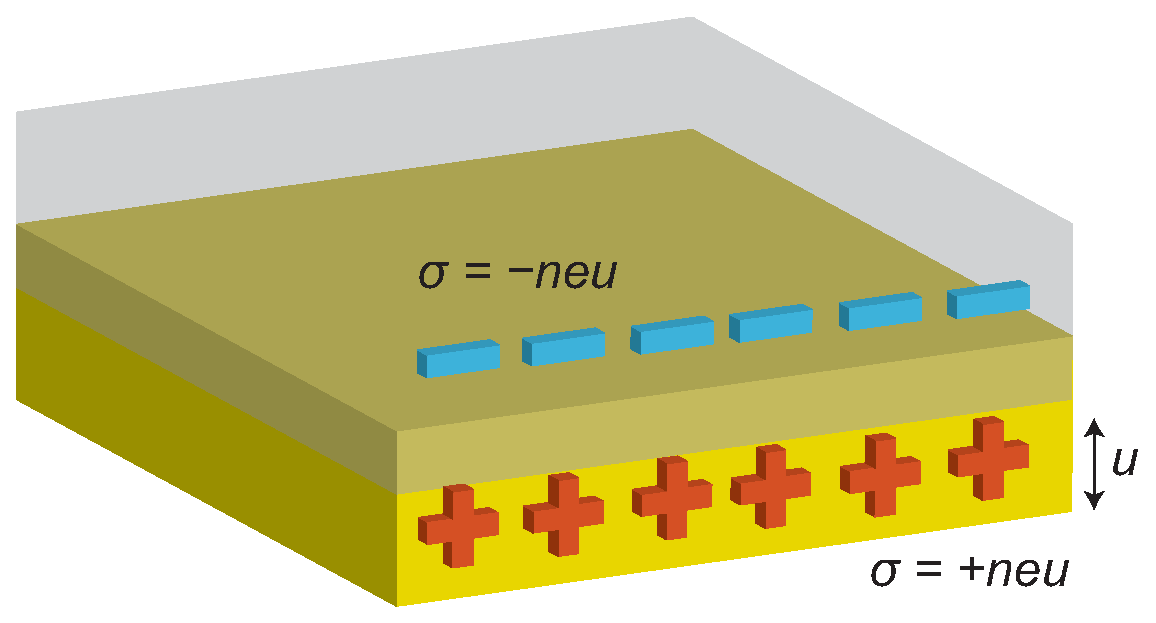
\includegraphics[scale=0.5]{THM/bulk.eps}
\caption{\label{fig:bulk}Longitudinal collective oscillations of the conduction electrons of a metal (Volume plasmons)}
\end{figure}
 We can derive plasma frequency $\omega_p$ from the simple harmonics oscillation model, a collective displacement of the electron cloud by a distance $u$ leads to a surface charge density $\sigma = \pm neu$ at the slab boundaries. This establishes a homogeneous electric field $\mathbf{E} = \frac{neu}{\varepsilon_0}$ inside the slab. Thus, the displaced electrons experience a restoring force, and their movement can be described by the equation of motion $nm\ddot{u} = -ne\mathbf{E}$. Inserting the expression for the electric field, this leads to
 \begin{subequations}
 \begin{align}
 nm\ddot{u} = -\frac{n^2e^2u}{\varepsilon_0} \\
 \ddot{u} + {\omega_p}^{2}u = 0\text{.}
 \end{align}
 \end{subequations}
  The plasma frequency $\omega_p = \sqrt{\frac{ne^2}{\varepsilon_0m}}$ can thus be recognized as the natural frequency of a free oscillation of the electron sea. The quanta of these charge oscillations are called plasmons. Due to the longitudinal nature of the excitation, volume plasmons do not couple to transverse electromagnetic waves, and can only be excited by particle impact. We can derive the dispersion relation of the generalization of volume plasmons, traveling plasma waves, from curl electric field equations (Equations~\ref{eq:curlE})
 \begin{subequations}
 \begin{align}
 \curl{\curl \mathbf{E}} &= -\mu_0 \frac{\partial^2\mathbf{D}}{\partial t^2}\label{eq:curlE}\\
\mathbf{K}( \mathbf{K}\cdot \mathbf{E}-K^{ 2 }\mathbf{E} ) &=-\varepsilon ( \mathbf{K},\omega  ) \frac { { \omega  }^{ 2 } }{ { c }^{ 2 } } \mathbf{E}
 \end{align}
 \end{subequations}  
and plasma model, and a simple equation of motion for an electron of the plasma subjected to an external electric field $\mathbf{E}$
 \begin{equation}
m\ddot{\mathbf{x}} + m\gamma\dot{\mathbf{x}} = -e\mathbf{E}\text{.}
\end{equation}
Assuming a harmonic time dependence $\mathbf{E}( t )=\mathbf{E}_0\mathrm{e}^{-i\omega t}$ of the driving field, a particular solution of this equation describing the oscillation of the electron is $\mathbf{x} ( t ) = \mathbf{x}_0 \mathrm{e}^{-i\omega t} $. The complex amplitude $\mathbf{x}_0$ incorporates any phase shifts between driving field and response via
\begin{equation}
\mathbf{x} ( t ) = \frac{e}{m( \omega^2 + i\gamma\omega )}\mathbf{E}( t )\text{.}
\end{equation}
The displaced electrons contribute to the macroscopic polarization
\begin{equation}
\mathbf{P}=-\frac{ne^2}{m( \omega^2 + i\gamma\omega )}\mathbf{E}( t )\text{.}
\end{equation}
Inserting $\mathbf{P}$ into dielectric displacement field equation $\mathbf{D} = \varepsilon_0\mathbf{E} + \mathbf{P}$ yields
\begin{equation}
\mathbf{D} = \varepsilon_0(1-\frac{\omega_p^2}{\omega^2 + i\gamma\omega})\mathbf{E}\text{,}
\end{equation}
where $\omega_p^2 = \frac{ne^2}{\varepsilon_0m}$. Therefore, the dielectric function of the free electron gas
\begin{equation}
\varepsilon(\omega) = 1- \frac{\omega_p^2}{\omega^2 + i\gamma\omega}\text{.}\label{eq:dielefu}
\end{equation}
We arrive at the desired result by using equation~\ref{eq:dielefu} and the generic dispersion relation $K^2=\varepsilon(\mathbf{K},\omega)\frac{\omega^2}{c^2}$, the dispersion relation of traveling waves becomes
\begin{equation}
\omega^2 = \omega_p^2 + \mathbf{K}^2c^2\text{.}
\end{equation}
From this relation, we can figure out the oscillation properties in any frequency of external field. Note that this branch can not confine the electromagnetic waves, it would radiate out the energy, so this mode is also called radiative surface plasmon.

\section{Surface plasmon polaritons at interface between dielectric and metal}

Surface plasmon polaritons (SPPs) are eigenmodes of transverse magnetic (TM) waves, which coupling the electromagnetic fields to oscillations of the conductor's electron plasma, propagate at a interface between dielectric and metal, and are confined in perpendicular direction. Providing a flat interface between dielectric and metal half-spaces with dielectric constants $\varepsilon_d$ and $\varepsilon_m$ , respectively, and assuming the interface normal to z direction and the SPPs propagate along the $x$ direction, the SPP wave vector $\beta$ is related to the frequency $\omega$ through the dispersion relation
\begin{equation}
\beta = k_0\sqrt{\frac{\varepsilon_d\varepsilon_m}{\varepsilon_d + \varepsilon_m}}\text{,}\label{eq:sppsdisp}
\end{equation}
where $k_0 = \omega/c$ is the free-space wave vector. We take $\omega$ to be real and allow $\beta$ to be complex.

The optical response of metals is often described by the Drude model for a free-electron gas~\cite{kittel1976introduction},
\begin{equation}
\varepsilon_{Drude}(\omega)=1-\frac{\omega_p^2}{\omega^2+i\Gamma\omega}\text{,}
\end{equation}
in which $\Gamma$ is a damping rate due to electron-electron and electron-phonon scattering.
Figure~\ref{fig:SPPdisp} shows the dispersion curve~\ref{eq:sppsdisp} with Drude metal  in the absence of losses ($\Gamma=0$) for air ($\varepsilon_d = 1$) and fused silica ($\varepsilon_d = 2.25$) interface.
\begin{figure}[htb]
\centering
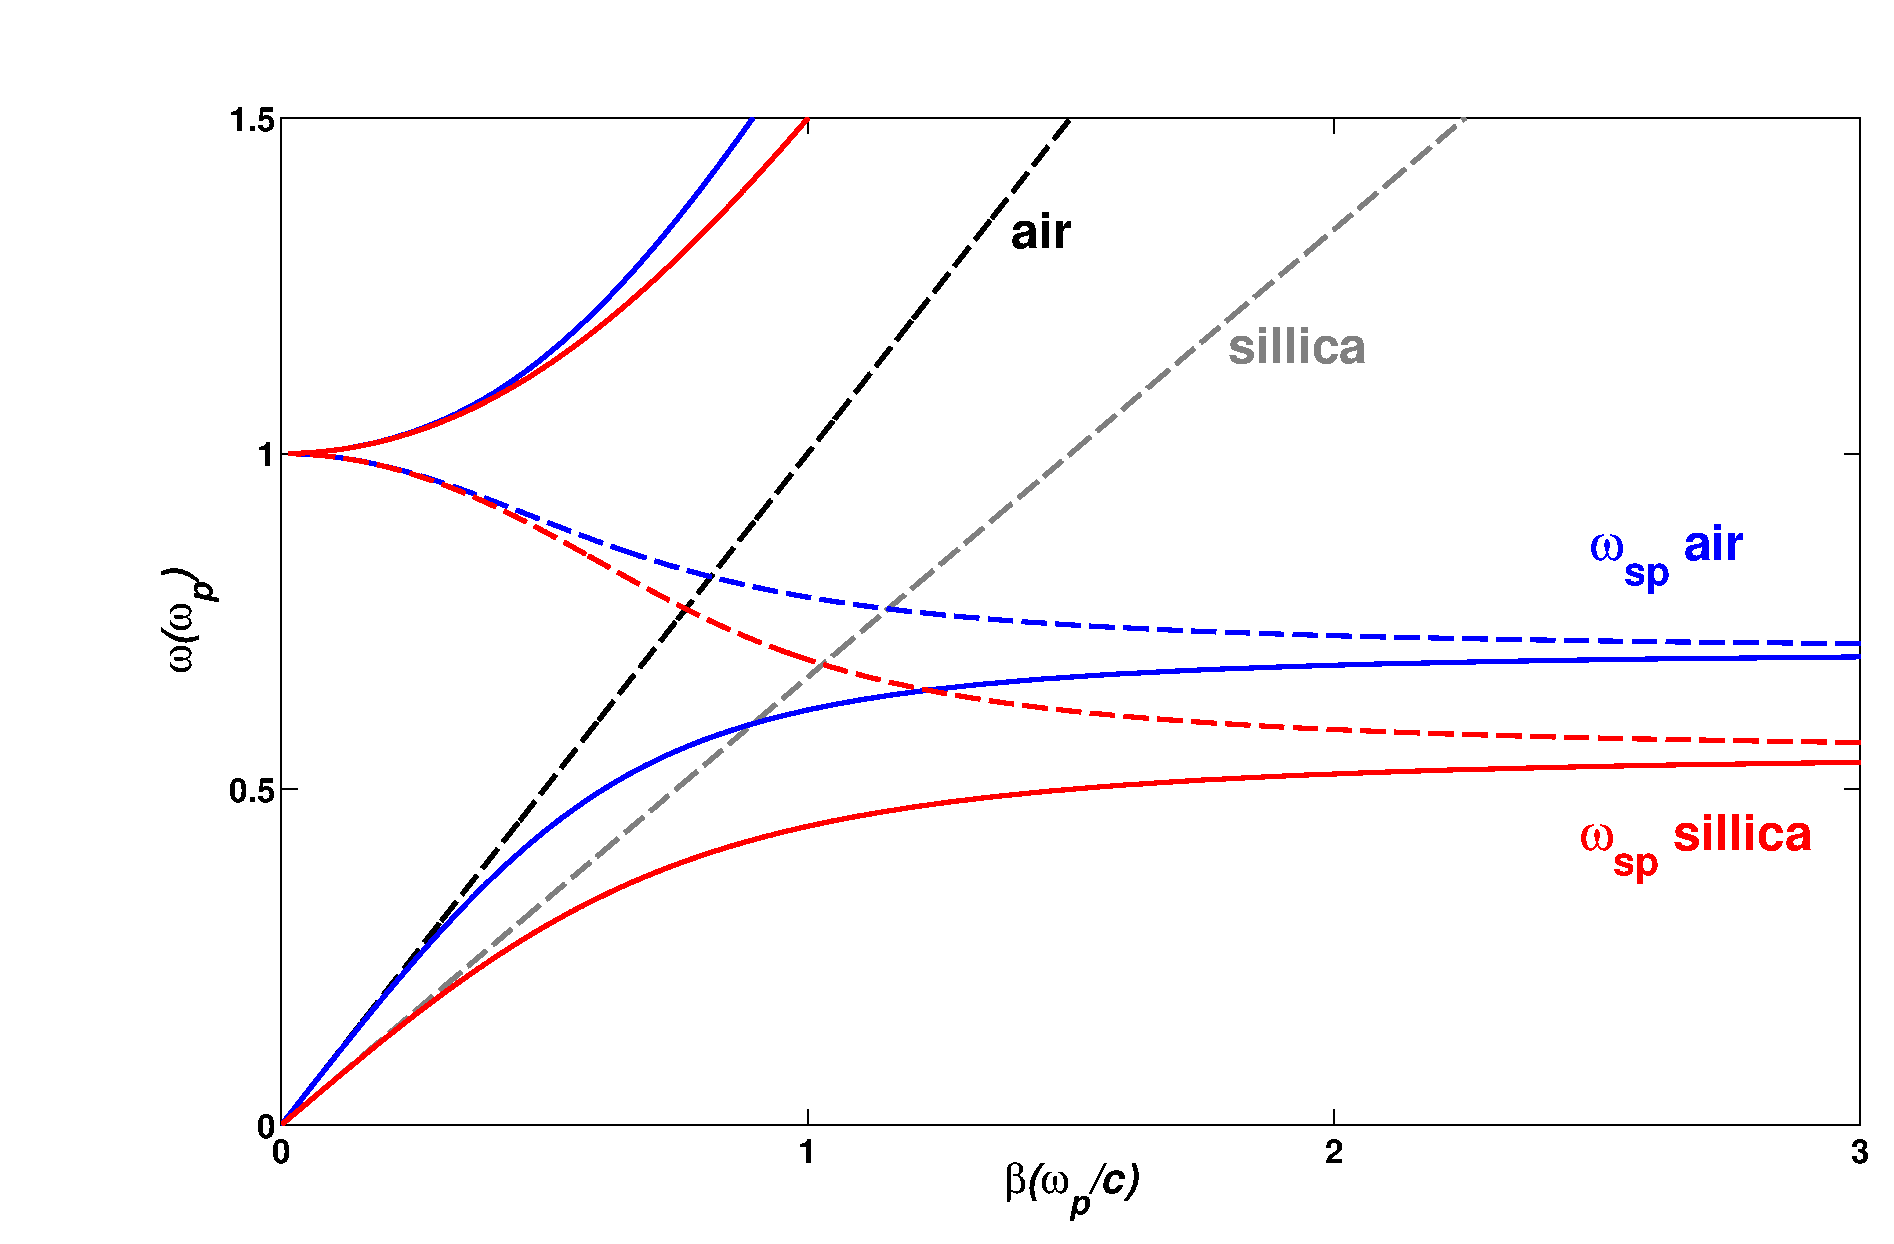
\includegraphics[scale=0.4]{THM/SPPdisp.eps}
\caption{\label{fig:SPPdisp}Dispersion relation of SPPs at the interface between a Drude metal with negligible collision frequency and air (blue curves) and silica (red curves).}
\end{figure}
For small wave vectors SPPs propagation constant $\beta$ is close to $k_0$ at the light line, in the opposite regime of the frequency close to surface plasmon frequency $\omega_p$. It also shows that the SPPs line lying to the right of the respective light lines of air and silica, so that SPPs are directed by light due to phase mismatching. The wave vector mismatch between SPPs and radiation modes needs to be overcome in order to excite or detect SPPs. This can be achieved by multiple methods~\cite{raether1988surface}. In the Otto configuration, light in a prism that is brought in close vicinity to a metal surface can excite SPPs through coupling to the evanescent field. Because light in the prism has a larger wave vector than that in air, it can be phase-matched to the SPPs. In the related Kretschmann-Raether geometry, coupling to SPPs occurs through a metal film that is deposited on a prism. In the grating coupling configuration, metal surface with a shallow grating of grooves or holes with lattice constant $a$. For the simple 1D grating of grooves depicted in Figure~\ref{fig:grating},
\begin{figure}[htb]
\centering
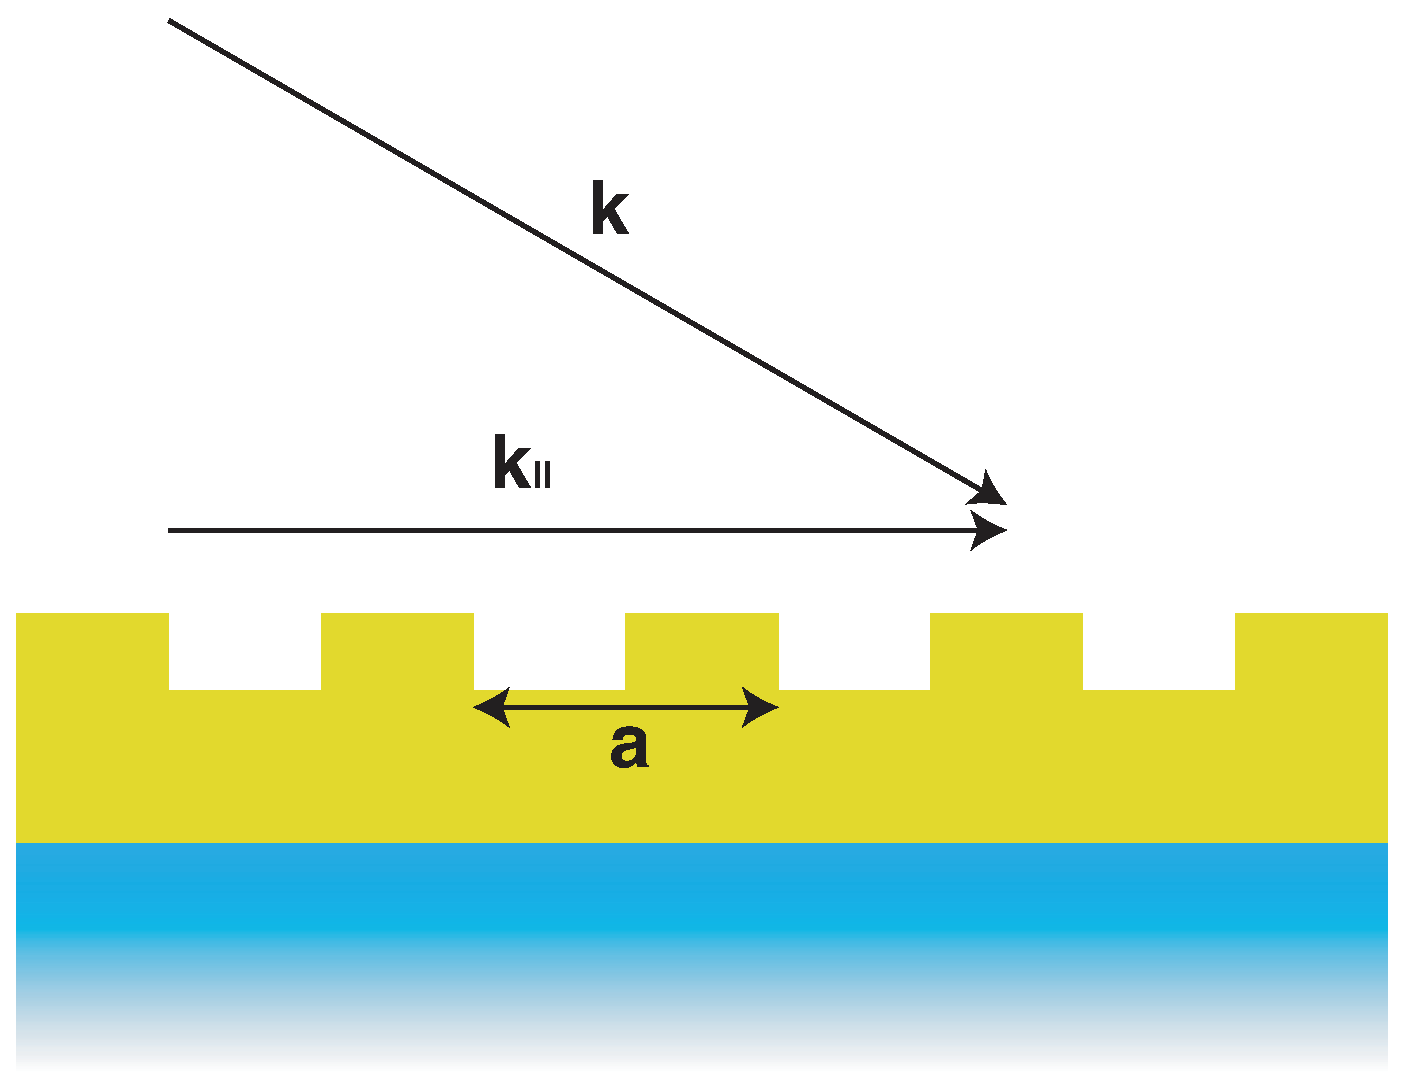
\includegraphics[scale=0.5]{THM/grating.eps}
\caption{\label{fig:grating}Phase-matching of light to SPPs the grating coupling configuration.}
\end{figure}
phase-matching takes place when the condition is fulfilled
\begin{equation}
\beta = k_0 \sin{\theta} \pm \nu g\text{,}
\end{equation}
where $g=\frac{2\pi}{a}$ is the reciprocal vector of the grating, and $\nu=(1,2,3\dots)$.
As with prism coupling, excitation of SPPs is detected as a minimum in the reflected light. The reverse process can also take place, SPPs propagating along a surface modulated with a grating can couple to light and thus radiate. 

%\bibliographystyle{unsrt}
%\bibliography{thesisbib}           =>  \chapter{Theory of surface plasmon polaritons in metallic nano-structures}
\label{c:thm}
\section{Definition of plasmon}

Plasmon is collective oscillation of conduction electron gas, a quasi-particle resulting from the quantization of plasma oscillations just like phonons are quantizations of mechanical vibrations. The simplest case is the volume plasmon as shown in Figure~\ref{fig:bulk}.
\begin{figure}[htb]
\centering
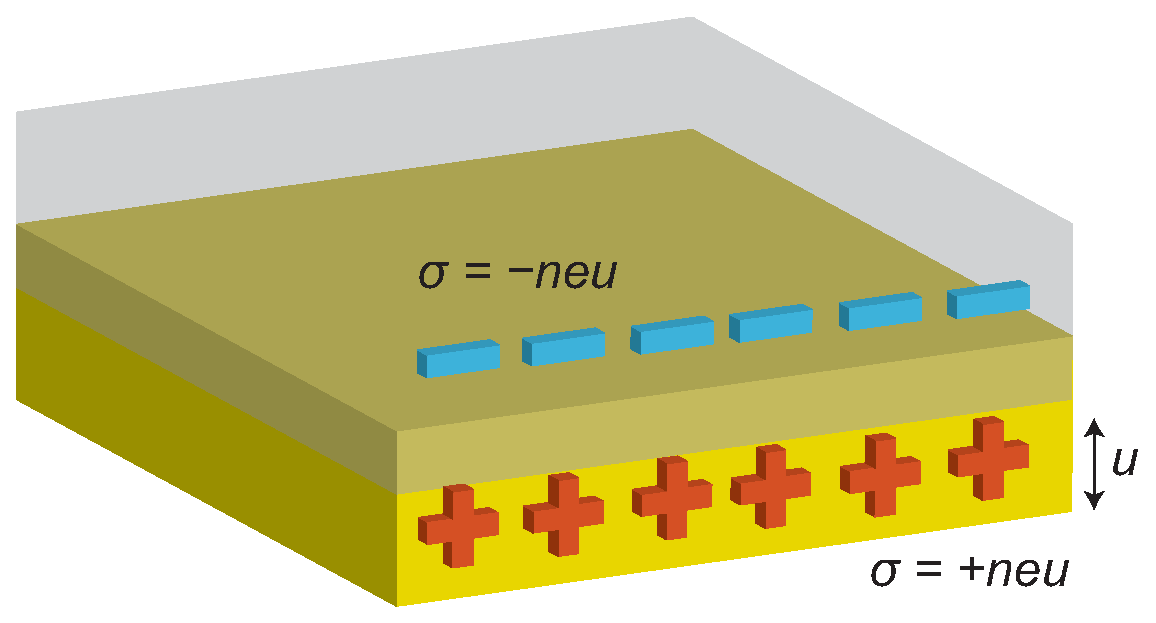
\includegraphics[scale=0.5]{THM/bulk.eps}
\caption{\label{fig:bulk}Longitudinal collective oscillations of the conduction electrons of a metal (Volume plasmons)}
\end{figure}
 We can derive plasma frequency $\omega_p$ from the simple harmonics oscillation model, a collective displacement of the electron cloud by a distance $u$ leads to a surface charge density $\sigma = \pm neu$ at the slab boundaries. This establishes a homogeneous electric field $\mathbf{E} = \frac{neu}{\varepsilon_0}$ inside the slab. Thus, the displaced electrons experience a restoring force, and their movement can be described by the equation of motion $nm\ddot{u} = -ne\mathbf{E}$. Inserting the expression for the electric field, this leads to
 \begin{subequations}
 \begin{align}
 nm\ddot{u} = -\frac{n^2e^2u}{\varepsilon_0} \\
 \ddot{u} + {\omega_p}^{2}u = 0\text{.}
 \end{align}
 \end{subequations}
  The plasma frequency $\omega_p = \sqrt{\frac{ne^2}{\varepsilon_0m}}$ can thus be recognized as the natural frequency of a free oscillation of the electron sea. The quanta of these charge oscillations are called plasmons. Due to the longitudinal nature of the excitation, volume plasmons do not couple to transverse electromagnetic waves, and can only be excited by particle impact. We can derive the dispersion relation of the generalization of volume plasmons, traveling plasma waves, from curl electric field equations (Equations~\ref{eq:curlE})
 \begin{subequations}
 \begin{align}
 \curl{\curl \mathbf{E}} &= -\mu_0 \frac{\partial^2\mathbf{D}}{\partial t^2}\label{eq:curlE}\\
\mathbf{K}( \mathbf{K}\cdot \mathbf{E}-K^{ 2 }\mathbf{E} ) &=-\varepsilon ( \mathbf{K},\omega  ) \frac { { \omega  }^{ 2 } }{ { c }^{ 2 } } \mathbf{E}
 \end{align}
 \end{subequations}  
and plasma model, and a simple equation of motion for an electron of the plasma subjected to an external electric field $\mathbf{E}$
 \begin{equation}
m\ddot{\mathbf{x}} + m\gamma\dot{\mathbf{x}} = -e\mathbf{E}\text{.}
\end{equation}
Assuming a harmonic time dependence $\mathbf{E}( t )=\mathbf{E}_0\mathrm{e}^{-i\omega t}$ of the driving field, a particular solution of this equation describing the oscillation of the electron is $\mathbf{x} ( t ) = \mathbf{x}_0 \mathrm{e}^{-i\omega t} $. The complex amplitude $\mathbf{x}_0$ incorporates any phase shifts between driving field and response via
\begin{equation}
\mathbf{x} ( t ) = \frac{e}{m( \omega^2 + i\gamma\omega )}\mathbf{E}( t )\text{.}
\end{equation}
The displaced electrons contribute to the macroscopic polarization
\begin{equation}
\mathbf{P}=-\frac{ne^2}{m( \omega^2 + i\gamma\omega )}\mathbf{E}( t )\text{.}
\end{equation}
Inserting $\mathbf{P}$ into dielectric displacement field equation $\mathbf{D} = \varepsilon_0\mathbf{E} + \mathbf{P}$ yields
\begin{equation}
\mathbf{D} = \varepsilon_0(1-\frac{\omega_p^2}{\omega^2 + i\gamma\omega})\mathbf{E}\text{,}
\end{equation}
where $\omega_p^2 = \frac{ne^2}{\varepsilon_0m}$. Therefore, the dielectric function of the free electron gas
\begin{equation}
\varepsilon(\omega) = 1- \frac{\omega_p^2}{\omega^2 + i\gamma\omega}\text{.}\label{eq:dielefu}
\end{equation}
We arrive at the desired result by using equation~\ref{eq:dielefu} and the generic dispersion relation $K^2=\varepsilon(\mathbf{K},\omega)\frac{\omega^2}{c^2}$, the dispersion relation of traveling waves becomes
\begin{equation}
\omega^2 = \omega_p^2 + \mathbf{K}^2c^2\text{.}
\end{equation}
From this relation, we can figure out the oscillation properties in any frequency of external field. Note that this branch can not confine the electromagnetic waves, it would radiate out the energy, so this mode is also called radiative surface plasmon.

\section{Surface plasmon polaritons at interface between dielectric and metal}

Surface plasmon polaritons (SPPs) are eigenmodes of transverse magnetic (TM) waves, which coupling the electromagnetic fields to oscillations of the conductor's electron plasma, propagate at a interface between dielectric and metal, and are confined in perpendicular direction. Providing a flat interface between dielectric and metal half-spaces with dielectric constants $\varepsilon_d$ and $\varepsilon_m$ , respectively, and assuming the interface normal to z direction and the SPPs propagate along the $x$ direction, the SPP wave vector $\beta$ is related to the frequency $\omega$ through the dispersion relation
\begin{equation}
\beta = k_0\sqrt{\frac{\varepsilon_d\varepsilon_m}{\varepsilon_d + \varepsilon_m}}\text{,}\label{eq:sppsdisp}
\end{equation}
where $k_0 = \omega/c$ is the free-space wave vector. We take $\omega$ to be real and allow $\beta$ to be complex.

The optical response of metals is often described by the Drude model for a free-electron gas~\cite{kittel1976introduction},
\begin{equation}
\varepsilon_{Drude}(\omega)=1-\frac{\omega_p^2}{\omega^2+i\Gamma\omega}\text{,}
\end{equation}
in which $\Gamma$ is a damping rate due to electron-electron and electron-phonon scattering.
Figure~\ref{fig:SPPdisp} shows the dispersion curve~\ref{eq:sppsdisp} with Drude metal  in the absence of losses ($\Gamma=0$) for air ($\varepsilon_d = 1$) and fused silica ($\varepsilon_d = 2.25$) interface.
\begin{figure}[htb]
\centering
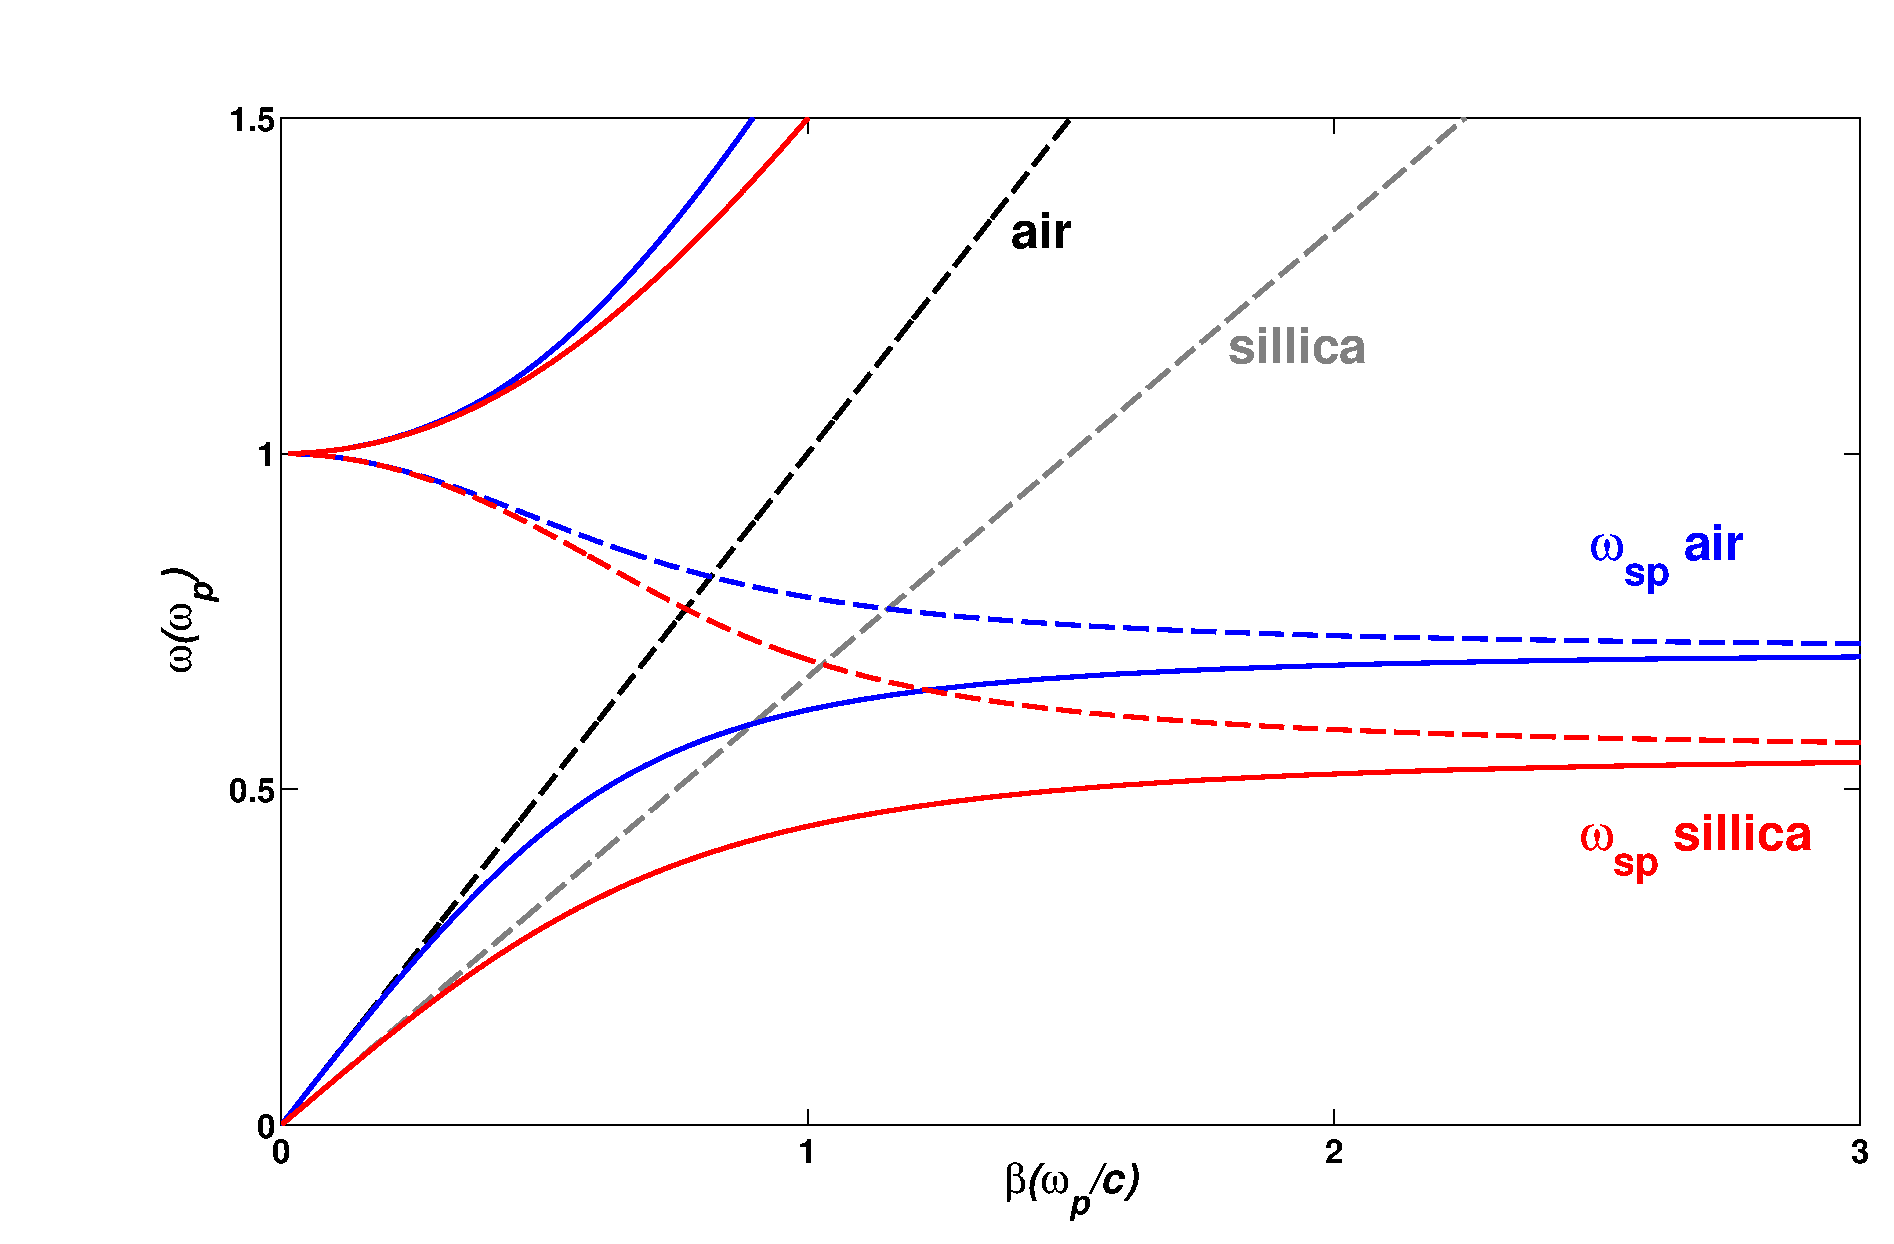
\includegraphics[scale=0.4]{THM/SPPdisp.eps}
\caption{\label{fig:SPPdisp}Dispersion relation of SPPs at the interface between a Drude metal with negligible collision frequency and air (blue curves) and silica (red curves).}
\end{figure}
For small wave vectors SPPs propagation constant $\beta$ is close to $k_0$ at the light line, in the opposite regime of the frequency close to surface plasmon frequency $\omega_p$. It also shows that the SPPs line lying to the right of the respective light lines of air and silica, so that SPPs are directed by light due to phase mismatching. The wave vector mismatch between SPPs and radiation modes needs to be overcome in order to excite or detect SPPs. This can be achieved by multiple methods~\cite{raether1988surface}. In the Otto configuration, light in a prism that is brought in close vicinity to a metal surface can excite SPPs through coupling to the evanescent field. Because light in the prism has a larger wave vector than that in air, it can be phase-matched to the SPPs. In the related Kretschmann-Raether geometry, coupling to SPPs occurs through a metal film that is deposited on a prism. In the grating coupling configuration, metal surface with a shallow grating of grooves or holes with lattice constant $a$. For the simple 1D grating of grooves depicted in Figure~\ref{fig:grating},
\begin{figure}[htb]
\centering
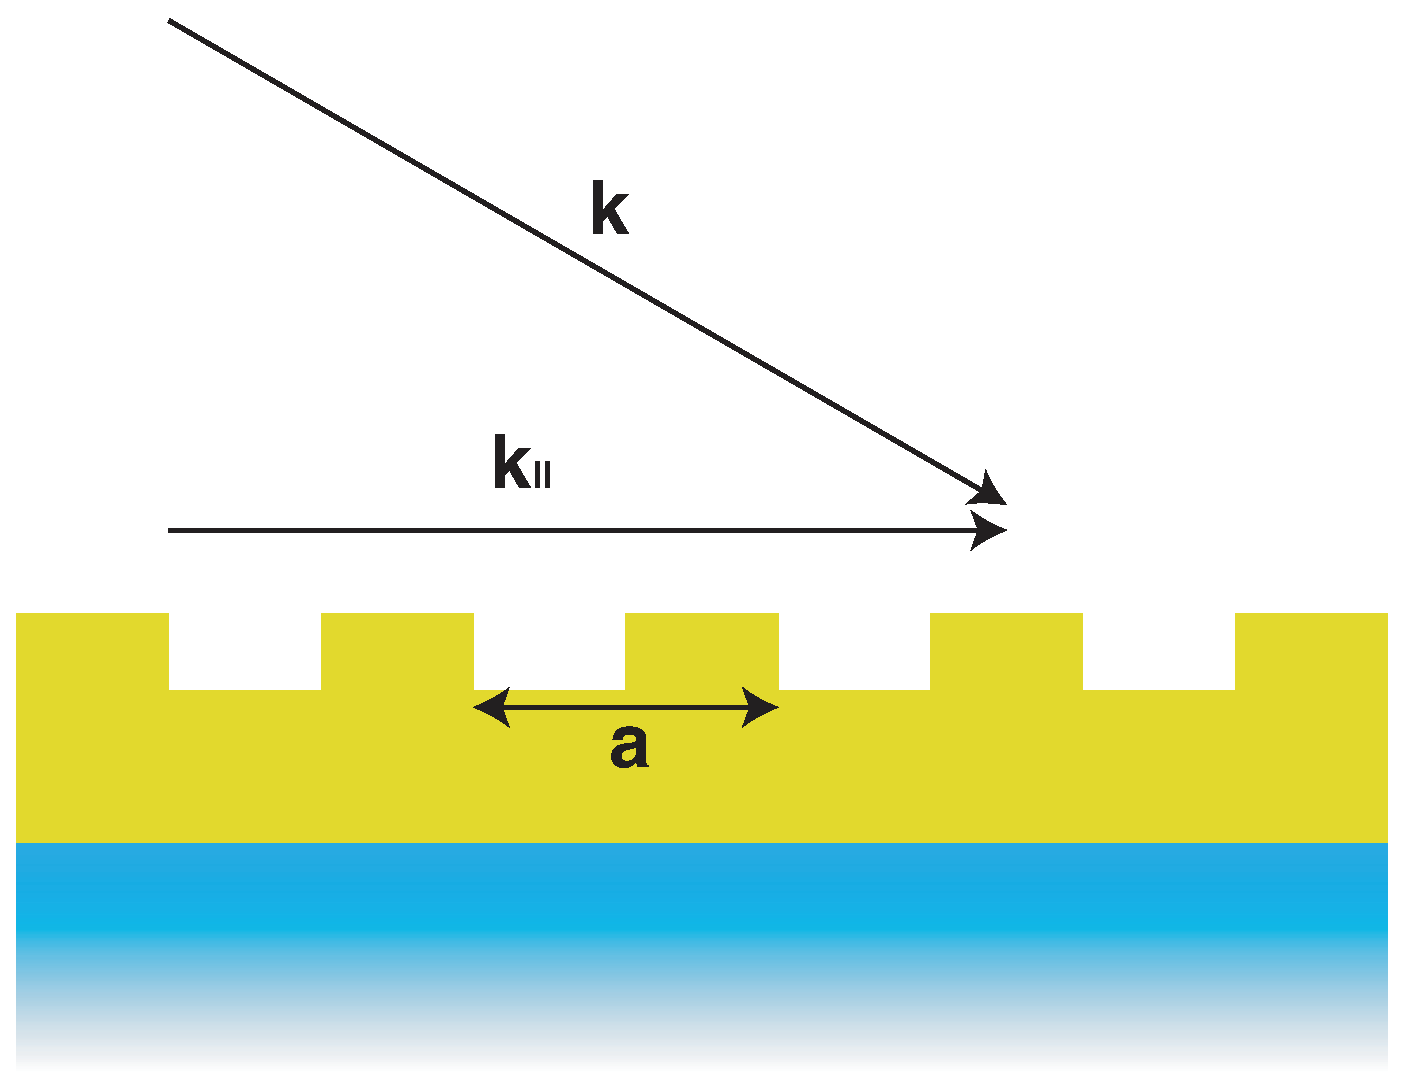
\includegraphics[scale=0.5]{THM/grating.eps}
\caption{\label{fig:grating}Phase-matching of light to SPPs the grating coupling configuration.}
\end{figure}
phase-matching takes place when the condition is fulfilled
\begin{equation}
\beta = k_0 \sin{\theta} \pm \nu g\text{,}
\end{equation}
where $g=\frac{2\pi}{a}$ is the reciprocal vector of the grating, and $\nu=(1,2,3\dots)$.
As with prism coupling, excitation of SPPs is detected as a minimum in the reflected light. The reverse process can also take place, SPPs propagating along a surface modulated with a grating can couple to light and thus radiate. 

%\bibliographystyle{unsrt}
%\bibliography{thesisbib}
\chapter{Experiment}
\label{c:exp}

\section{Experiment Setup} % (fold)
\label{s:experiment_setup}

In this section, we discuss the resluts of our experiments.  There are four parts in our experiments.  First, we compare our framework with other frameworks in the communication cost.  Second, since there are several stages of improvement in our framework, we discuss each of their influence to our final model.  Third, we consider the amortization of transmitting the orthogonal matrices.  Finally, we compare the power of pruning among different bounds.  For every experiment, we collect the results of $100$ experiments by randomly picking our $100$ instances as the queries.
% section experiment_setup (end)

\section{Data Description} % (fold)
\label{s:data_description}

The table \ref{table:datasets} is the description of those datasets we used in our experiments. Note that the $n\times m$ in the final column means that there are $n$ instances placed in each machine and $m$ machines used in this experiments.  For instance, for the image dataset ANN with SIFT feature, there are totally $5000$ machines and each has $200$ instances in our experiments.

\begin{table}[htpb]\begin{center}
\caption{Summary for each dataset}\label{table:datasets}
\begin{tabular}{|c|c|c|c|c|}
\hline 
Type & Dataset & Feature & Num of Dimensions & Num of Instances\\ \hline \hline
Time Series & Random Walk & $N(0,1)$ & 128 & $200\times 5000$\\ \hline
\multirow{3}{*}{Image} & ANN & SIFT & 128 & $200\times 5000$\\ 
\cline{2-5}
 & \multirow{2}{*}{Flickr} & CSD & 256 & $500\times 2000$\\ 
\cline{3-5}
 & & SCD & 256 & $500\times 2000$\\ \hline
 \multirow{2}{*}{Audio} & \multirow{2}{*}{Million Songs} & MVD & 480 & $500\times 1900$ \\ 
 \cline{3-5}
 & & TRH & 480 & $500\times 1900$\\ \hline
\end{tabular}
\end{center}\end{table}

\subsection{Time Series Data} % (fold)
\label{ssb:time}
The time series datasets we used is a synthetic dataset.  We use the random walk data model in \cite{time}.  Each time series is generated by a random walk whose every step size is a normal distributed random number with mean $0$ and standard deviation $1$.  We also use this model to generate the synthetic dataset in the experiments of MsWave \cite{MsWave}.
% subsection time (end)

\subsection{Image Data} % (fold)
\label{ss:Image}
We use two datasets in our experiments for images.  First is the data provied in \cite{ANN}, which is a widely used dataset for evaluate the performance of approximate nearest neighbors search algorithms.  The another one is the Flickr datasets with two kind of features used in \cite{Flickr}.  The dataset is also a widely used dataset in the task of image retrieval.  The CSD indicates \emph{Color Structure Descriptor} while the SCD means \emph{Scalable Color Descriptor}.
% subsection Image (end)

\subsection{Audio Data} % (fold)
\label{sub:audio_data}
Here we use the audio data named Million Song Dataset from~\cite{Bertin-Mahieux2011} which is a free-available collection of audio features for a million contemporary popular music tracks. For the features, MVD means \emph{Modulation Frequency Variance Descriptor} and TRH is \emph{Temporal Rhythm Histograms}.  Please refer to \cite{LID_05ismir,RAU_03jnmr,RAU_01ecdl} to see the details about how these features were extracted.
% subsection audio_data (end)

% subsection data_description (end)

\section{Comparison Among all Frameworks} % (fold)
\label{s:comparison_among_all_frameworks}

\subsection{Frameworks for Comparison} % (fold)
\label{ss:frameworks_for_comparison}

We compare our framework with those methods mentioned in the related work chapter.  From \cite{PRP}, we use CP and PRP but with slightly modifications. In the origin CP, every machine would return the top $k$ instances once receiving the query.  But there is a trivial improvement that every machine only return the \emph{distances} of these top $k$ instances.  Then, the server could know the distances of the $k$NN of this query and then ask those machines with answers to return those instances.  Although it is a slight modification, it could reduce the cost of CP a lot when the number of machines is large.  Also, we run LeeWave \cite{LeeWave} in these experiments for comparision.  We call our final framework as \emph{Main} in the following figures.


Note that in the following experiments, the cost of our framework here does not include the cost of sending the orthogonal matrices.  We will prove in the section~\ref{s:number_of_queries_for_amortizing_the_cost_of_matrices} that the total cost including the matrices could be amortized by enough queries and thus to achieve the cost here.  That is, we could see the cost of our framework here as the cost after amortized by enough queries.  Due to the time limitations, we didn't conduct enough number of queries to achieve the amortized results for each dataset.


% subsection frameworks_for_comparison (end)

\subsection{Results of Different Frameworks} % (fold)
\label{sub:results_of_different_fra}

The following figures are the results of our experiments.  The $x$ axis indicates the number of local machines while the $y$ axis is the total transmission cost of the 100 queries.  Since the differences among these are too large, we transform the $y$ axis to logarithmic scale.  

\begin{figure}[htpb!]
  \centering
  \includegraphics[width=1.0\linewidth]{exp/out/time.png}
  \caption{Different Frameworks on Time Series}
  \label{fig:out_time}
\end{figure}

\begin{figure}[htpb!]
  \centering
  \includegraphics[width=1.0\linewidth]{exp/out/ANN.png}
  \caption{Different Frameworks on ANN}
  \label{fig:out_ANN}
\end{figure}

\begin{figure}[htpb!]
  \centering
  \includegraphics[width=1.0\linewidth]{exp/out/f2.png}
  \caption{Different Frameworks on Flickr:~CSD}
  \label{fig:out_f2}
\end{figure}

\begin{figure}[htpb!]
  \centering
  \includegraphics[width=1.0\linewidth]{exp/out/f3.png}
  \caption{Different Frameworks on Flickr:~SCD}
  \label{fig:out_f3}
\end{figure}

\begin{figure}[htpb!]
  \centering
  \includegraphics[width=1.0\linewidth]{exp/out/mvd.png}
  \caption{Different Frameworks on Million Song:~MVD}
  \label{fig:out_mvd}
\end{figure}

\begin{figure}[htpb!]
  \centering
  \includegraphics[width=1.0\linewidth]{exp/out/trh.png}
  \caption{Different Frameworks on Million Song:~TRH}
  \label{fig:out_trh}
\end{figure}

From these figures, we could see that our framework used the least transmission cost among all these frameworks for every dataset.  And these differences between our framework and each other framework increased as the number of local machines increased.  The reason is that when the number of local machines increases, there would be a higher chance to prune more local machines in the early round since the ratio of pruned machines doesn't change too much.  But the other frameworks would be more sensitive to the number of local machines.


The performance of CP and PRP are similar to each other in most dataset.  It is because when $k$ is much smaller than the number of total local machines, their procedure would be almost the same except the final stage.  For those cases where PRP is worse than CP, we could find that PRP would return too many instances in the final stage while CP would only return exact $k$ instances back to the server.  But these results would highly depend on the distribution of the instances among these local machines and could not be controled by the algorithms themself.


We could also notice that LeeWave needs the largest transmission cost to finding the $k$NN for the $100$ queries for all datasets.  When the type of the dataset is time series (figure \ref{fig:out_time}), the different between LeeWave and other frameworks are smaller than other datasets since its pruning power is still effective for this type of dataset. For other types of datasets like images or audio, LeeWave almost could not prune any candidiate machines until the last round which would sent the whole query to each machine and thus used a large amount of transmission cost. 

Even though the LeeWave could prune some candidates machines when the type of the dataset is time series, there is a big gap between it and CP, PRP.  The reason of the large transmission cost in LeeWave here is not the pruning power but its way to calculate the bounds.  In each round, after sending the coefficients in this level of the error tree, LeeWave requires every instances to return some metadata back for calculating the bounds at the server.  This causes one term in the transmission cost of LeeWave would grows linearly with the total number of instances in all local machines.  Since we conducted our experiments on the datasets with about one million instances, this term would be large enough to cover the saving from the pruning.  On the other hand, the transmission cost of CP and PRP is independent of the total number of instance but only dependent on the number of local machines and $k$.  Therefore, when the total instances is large, LeeWave could use more transmission cost than CP and PRP even when its pruning power still exists.


% subsection results_of_different_fra (end)	
% section comparison_among_all_frameworks (end)



\section{Comparison Among our Framework with Different Configurations} % (fold)
\label{s:comparison_among_our_framework_with_different_configurations}


\subsection{Configurations for Comparison} % (fold)
\label{sub:configurations_for_comparison}

There are many stages of algorithms which build the final version of our framework.  Therefore, in this section, we would like to discuss the performance of our framwork with or without each of these algorithms.  We conducted the experiments for the following different configurations of our framework.

\emph{Main}: It is the final version of our framework which obtains all algorithms mentioned in the chapter of methodology.

\emph{NoW}: To test the influence of the orthogonal transformation, we consider the configuration which has all the algorithms except the orthogonal transmission.  We could take it as the special case of \emph{Main} where $W_i=I,~\forall i=1,2,\ldots,m$.

\emph{NoPRP}: In the section~\ref{ss:find_the_threshold_in_distributed_machines}, we use PRP to find the threshold for pruning in each round.  Therefore, we want to compare this modification with the original version which directly returns all bounds back to the server.

\emph{NoCD}: In the section~\ref{ss:coordinate_descent_to_decide_the_pivots}, the number of dimensions we sent for every query are decided dynamically by solving an optimization problem with Coordinate Descent.  Here we just send $10\%$ of the transformed query in each round to the server for comparing the improvement from the optimiaztion.

% subsection configurations_for_comparison (end)

\subsection{Results of Different Configurations} % (fold)
\label{sub:results_of_different_configurations}


We provide the results of the experiments to compare our framework with different configurations in the following figures. The meanings of their axises are same with those in the section \ref{sub:results_of_different_fra}.

\begin{figure}[htpb!]
  \centering
  \includegraphics[width=1.0\linewidth]{exp/in/time.png}
  \caption{Different Configurations on Time Series}
  \label{fig:in_time}
\end{figure}

\begin{figure}[htpb!]
  \centering
  \includegraphics[width=1.0\linewidth]{exp/in/ANN.png}
  \caption{Different Configurations on ANN}
  \label{fig:in_ANN}
\end{figure}

\begin{figure}[htpb!]
  \centering
  \includegraphics[width=1.0\linewidth]{exp/in/f2.png}
  \caption{Different Configurations on Flickr:~CSD}
  \label{fig:in_f2}
\end{figure}

\begin{figure}[htpb!]
  \centering
  \includegraphics[width=1.0\linewidth]{exp/in/f3.png}
  \caption{Different Configurations on Flickr:~SCD}
  \label{fig:in_f3}
\end{figure}

\begin{figure}[htpb!]
  \centering
  \includegraphics[width=1.0\linewidth]{exp/in/mvd.png}
  \caption{Different Configurations on Million Song:~MVD}
  \label{fig:in_mvd}
\end{figure}

\begin{figure}[htpb!]
  \centering
  \includegraphics[width=1.0\linewidth]{exp/in/trh.png}
  \caption{Different Configurations on Million Song:~TRH}
  \label{fig:in_trh}
\end{figure}

In these figures, we could see that although every algorithm could make our framework better, their influences are very different to each other.  The algorithm which makes the largest difference with our final framework is PRP.  It is very obvious since we use PRP to find the threshold could make the transmission cost independent with the total number of instances.  This makes a big difference when the datasets here contain about one million instances.  The algortihm with the second big improvement is the orthogonal transformation.  This confirms our assumption that we could save transmission cost by improving the power of pruning with the help of the orthogonal transformation.  Finally, the algorithm of dynamically deciding the pivots with Coordinate Descent seems to have the least influence to our final framework in these figures.  However, it does contibute much to the saving of transmission even though not as significant as the others.  With the help of it, we don't have to worry about deciding the pivots for every dataset.

% subsection results_of_different_configurations (end)
% section configurations_for_comparison (end)

\section{Number of Queries for Amortizing the Cost of Matrices} % (fold)
\label{s:number_of_queries_for_amortizing_the_cost_of_matrices}

In the beginning of this chapter, we mentioned that the cost of our final framework showed in the previous experiments didn't count the cost of sending those orthogonal martices.  The matrices cost from the first phase of our framework is as below. 
\begin{equation}
\begin{aligned}
	Cost_{Matrix} & = m\times SingleMatrixCost \\
                  & = m\times \frac{D\times (D-1)}{2}
\end{aligned}
\end{equation}

where we have given the proof that we could use $\frac{D\times (D-1)}{2}$ parameters to represent an orthogonal matrix in the section \ref{ss:reduce_the_cost_of_sending_matrices}.


Although it would cause a large cost, it only needs to be done for one time.  Therefore, we could amortize it to the cost of every query in the second phase.  If the number of queries is large enough, we could amortize the matrices cost to a very small ratio of the total transmission cost.  But due to the time limitation, we didn't conduct the experiments for a large number of queries, therefore, we estimate the number of queries we need as below.

Given a small ratio (here we use $r_{ideal}=5\%$), we could estimate how many queries we need for amortizing the matrices cost to this ratio of the total transmission cost as below.  

\begin{equation}
\begin{aligned}
	Cost_{Total} & = & \sum_{t=1}^{\Vert Q\Vert}{Cost_{our}(q_t)} + Cost_{Matrix} \\
	Cost(i) & = & \frac{\sum_{t=1}^{\Vert Q\Vert}{Cost_{our}(q_t)}}{{\Vert Q\Vert}}\times i + Cost_{Matrix} \\
\end{aligned}
\end{equation}

In the equation above, we estimate the total cost of $i$ queries as $Cost_(i)$ by summing up the matrices cost and the average cost of the second phase in our past experiments multiplied by $i$.  In other words, we estimate the cost of the second phase for a single query as $\frac{\sum_{t=1}^{\Vert Q\Vert}{Cost_{our}(q_t)}}{{\Vert Q\Vert}}$. 

Therefore, our goal becomes how many queries we need to make the ratio of $Cost_{Matrix}$ lower than $r_{ideal}$.  We could write it as the following problem:

\begin{equation}\label{eq:amort}
\begin{aligned}
& \underset{i}{\text{minimize}}
~~\frac{Cost_{Matrix}}{Cost(i)} < r_{ideal} \\
& \text{where}~~i \in \mathbb{N}
\end{aligned}
\end{equation}

It could be solved easily.


\begin{table}[H]\begin{center}
\caption{Number of queries to amortize the cost of matrices}\label{table:amortize}
\begin{tabular}{|c|c|c|c|c|c|}
\hline 
Type & Dataset & Feature & Total Num of Instances & Num of Queries\\ \hline \hline
Time Series & Random Walk & $N(0,1)$ & $1000000$ & $4655$\\ \hline
\multirow{3}{*}{Image} & ANN & SIFT & $1000000$ & $1997$\\ 
\cline{2-5}
 & \multirow{2}{*}{Flickr} & CSD & $1000000$ & $6313$\\ 
 \cline{3-5}
 & & SCD &  $1000000$ & $12724$\\ \hline
 \multirow{2}{*}{Audio} & \multirow{2}{*}{Million Songs} & MVD & $950000$ & $6979$\\ 
 \cline{3-5}
 & & TRH & $950000$ & $7076$\\ \hline
\end{tabular}
\end{center}\end{table}

We solve~\eqref{eq:amort} for each dataset when the number of local machines reachs the maximal and $k=10$.  The results are put in the table \ref{table:amortize}.  From this table, we could find that although the matrices cost is large, we could amortize it to less than $5\%$ with a few thousands of queries.  For a dataset with one million of instances, the number of queries could be achieved easily.  


\begin{figure}[htpb!]
  \centering
  \includegraphics[width=1.0\linewidth]{exp/AQ/ANN.png}
  \caption{Pruning Results on Time Series}
  \label{fig:AQ}
\end{figure}

From the figure~\ref{fig:AQ}, we could notice that $\frac{Cost_{Matrix}}{Cost(i)} < r_{ideal}$ decreases fast as the number of queries increases.  As our estimation, this ratio achieve $5\%$ when the number of queries reach about $2000$.




% subsection number_of_queries_for_amortizing_the_cost_of_matrices (end)



\section{Power of the Pruning Procedure} % (fold)
\label{s:power_of_the_pruning_procedure}

\subsection{Methods with Different Bounds} % (fold)
\label{sub:methods_with_different_bounds}


There are three different bounds which we could compare.  The first one is the bounds of LeeWave, which comes from the Haar wavelet transformation.  The second one is the bounds we derived in the section~\ref{ss:derivation_of_the_bounds}.  That is the method \emph{NoW} we mentioned above.  The final bounds is those improved by the orthogonal transformation.


% subsection methods_with_different_bounds (end)


\subsection{Results of Pruning} % (fold)
\label{sub:results_of_pruning}

First, we compare the bounds we derived and the bounds of LeeWave.  Since the number of dimensions LeeWave sent in every round is restricted by the shape of the error tree, we could only compare the number of residual machines under these dimensions between LeeWave and our method.  For LeeWave, we just average the results of each query.  As for our method, we use our estimation for each dimension used in the section~\ref{ss:estimate_the_number_of_residual_machines} and pick those dimesions used in LeeWave.

From the table~\ref{table:time} for time series dataset, we could see that although LeeWave could prune some local machines in the last few round, our method outperforms it by pruning machines earlier and more.  This improvement mainly comes from our tighter bounds that provide a more powerful pruning mechanism.

\begin{table}[H]\begin{center}
\caption{Time Series, Number of residual machines after sending some dimensions for 5000 machines}\label{table:time}
\begin{tabular}{|c|c|c|c|c|c|c|c|c|}
\hline 
Method \textbackslash Dim & 2 & 4 & 8 & 16 & 32 & 64 & 128\\ \hline \hline
Ours & 4823.24 & 4469.71 & 3762.66 & 2344.46 & 540.14 & 69.11 & 9.99 \\ \hline
LeeWave & 4999.84 & 4984.90 & 4895.18 & 3722.49 & 938.80 & 111.00 & 9.99 \\ \hline
\end{tabular}
\end{center}\end{table}

However, for the other types of datasets, from these tables we could notice that LeeWave almost could not prune any local machine until the last round.  The reason is that since the bounds of LeeWave come from the Haar wavelet transformation, which is suitable for the time series feature, but not workable for the images and audio datasets from these experiments.  Although the power of pruning of our method would be different for different types of data, we could prune about half of total local machines after sending half of the query feature vector.  This allows us to avoid sending redundant information to unnecessary machines.


\begin{table}[H]\begin{center}
\caption{Flickr:CSD, Number of residual machines after sending some dimensions for 1000 machines}\label{table:f2}
\begin{tabular}{|c|c|c|c|c|c|c|c|c|c|}
\hline 
Method \textbackslash Dim & 2 & 4 & 8 & 16 & 32 & 64 & 128 & 256\\ \hline \hline
Ours & 995.37 & 986.10 & 967.56 & 930.49 & 856.34 & 573.79 & 410.3 & 9.89 \\ \hline
LeeWave & 1000 & 1000 & 1000 & 999.90 & 995.16 & 967.26 & 808.16 & 9.89 \\ \hline
\end{tabular}
\end{center}\end{table}


\begin{table}[H]\begin{center}
\caption{Million Songs: MVD, Number of residual machines after sending some dimensions for 800 machines}\label{table:mvd}
\begin{tabular}{|c|c|c|c|c|c|c|c|c|c|}
\hline 
Method \textbackslash Dim & 2 & 6 & 12 & 26 & 52 & 104 & 210 & 420\\ \hline \hline
Ours & 799.41 & 797.05 & 793.5 & 785.23 & 769.87 & 739.14 & 467.74 & 12.77 \\ \hline
LeeWave & 800 & 800 & 800 & 800 & 799.07 & 794.93 & 772.91 & 12.58 \\ \hline
\end{tabular}
\end{center}\end{table}


Finally, let's discuss the pruning power with or without the help of the orthogonal transformation, which is our final method and \emph{NoW}.  We plot our estimation in the section~\ref{ss:estimate_the_number_of_residual_machines} and compare their estimation.  However, we found that for some datasets, these could not reflect the status of pruning for \emph{NoW} since the decision of the pivots are concentrated in the latter part of the vector.  As a result, we add another method named \emph{NoCDW} which is same with \emph{NoW} but intead of dynamically deciding the pivots, it sends $10\%$ of the vector for each round.  In the following figures, the red circles are our final method, the black ones are \emph{NoW}, and the green ones are \emph{NoCDW}.

From the figure~\ref{fig:prune_ANN} and figure~\ref{fig:prune_trh}

For all these figures except the figure~\ref{fig:prune_f3}, we could see that our method could prune most of the residual machines with about $50\%$ of the total dimensions.  From \emph{NoCDW}, we could find we have to send many dimensions to prune some machines without the orthogonal transformation.  This difference comes from the tightness of the bounds.  After optimizing with the orthogonal transformation, our method could use much tighter bounds to prune machines than the original bounds.  With the enhanced prunine power, our method could save much transmission cost.

On the other hand, in the figure~\ref{fig:prune_ANN} and figure~\ref{fig:prune_trh}, the curve of \emph{NoW} is very different with \emph{NoCDW}.  The reason is that for these datasets, the pivots learnt from the estimation cost problem concentrate at the latter part of the vector, which leads to very poor estimation for residual machines for the earlier part of the vector.  So, its curve could not reflect the pruning power of the bounds without transformation.  This also implies the policy of sending $10\%$ total dimensions would not be the best policy for these datasets since the curve of \emph{NoW} is mcuh different with the one of \emph{NoCDW}.  For the other figures, we could see the curve of \emph{NoW} is similar with \emph{NoCDW}. This implies the $10\%$ policy would be fine for these datasets.  But since we could not know whether this policy would work for a dataset in advance, the best policy is to decide the pivots dynamically as we mentioned before.

\begin{figure}[htpb!]
  \centering
  \includegraphics[width=1.0\linewidth]{exp/prune/ANN.png}
  \caption{Pruning Results on ANN}
  \label{fig:prune_ANN}
\end{figure}

\begin{figure}[htpb!]
  \centering
  \includegraphics[width=1.0\linewidth]{exp/prune/f2.png}
  \caption{Pruning Results on Flickr:~CSD}
  \label{fig:prune_f2}
\end{figure}

\begin{figure}[htpb!]
  \centering
  \includegraphics[width=1.0\linewidth]{exp/prune/f3.png}
  \caption{Pruning Results on Flickr:~SCD}
  \label{fig:prune_f3}
\end{figure}

\begin{figure}[htpb!]
  \centering
  \includegraphics[width=1.0\linewidth]{exp/prune/mvd.png}
  \caption{Pruning Results on Million Song:~MVD}
  \label{fig:prune_mvd}
\end{figure}

\begin{figure}[htpb!]
  \centering
  \includegraphics[width=1.0\linewidth]{exp/prune/trh.png}
  \caption{Pruning Results on Million Song:~TRH}
  \label{fig:prune_trh}
\end{figure}


% subsection results_of_pruning (end)	


% section power_of_the_pruning_procedure (end)

%\bibliographystyle{unsrt}
%\bibliography{thesisbib}           =>  \chapter{Experiment}
\label{c:exp}

\section{Experiment Setup} % (fold)
\label{s:experiment_setup}

In this section, we discuss the resluts of our experiments.  There are four parts in our experiments.  First, we compare our framework with other frameworks in the communication cost.  Second, since there are several stages of improvement in our framework, we discuss each of their influence to our final model.  Third, we consider the amortization of transmitting the orthogonal matrices.  Finally, we compare the power of pruning among different bounds.  For every experiment, we collect the results of $100$ experiments by randomly picking our $100$ instances as the queries.
% section experiment_setup (end)

\section{Data Description} % (fold)
\label{s:data_description}

The table \ref{table:datasets} is the description of those datasets we used in our experiments. Note that the $n\times m$ in the final column means that there are $n$ instances placed in each machine and $m$ machines used in this experiments.  For instance, for the image dataset ANN with SIFT feature, there are totally $5000$ machines and each has $200$ instances in our experiments.

\begin{table}[htpb]\begin{center}
\caption{Summary for each dataset}\label{table:datasets}
\begin{tabular}{|c|c|c|c|c|}
\hline 
Type & Dataset & Feature & Num of Dimensions & Num of Instances\\ \hline \hline
Time Series & Random Walk & $N(0,1)$ & 128 & $200\times 5000$\\ \hline
\multirow{3}{*}{Image} & ANN & SIFT & 128 & $200\times 5000$\\ 
\cline{2-5}
 & \multirow{2}{*}{Flickr} & CSD & 256 & $500\times 2000$\\ 
\cline{3-5}
 & & SCD & 256 & $500\times 2000$\\ \hline
 \multirow{2}{*}{Audio} & \multirow{2}{*}{Million Songs} & MVD & 480 & $500\times 1900$ \\ 
 \cline{3-5}
 & & TRH & 480 & $500\times 1900$\\ \hline
\end{tabular}
\end{center}\end{table}

\subsection{Time Series Data} % (fold)
\label{ssb:time}
The time series datasets we used is a synthetic dataset.  We use the random walk data model in \cite{time}.  Each time series is generated by a random walk whose every step size is a normal distributed random number with mean $0$ and standard deviation $1$.  We also use this model to generate the synthetic dataset in the experiments of MsWave \cite{MsWave}.
% subsection time (end)

\subsection{Image Data} % (fold)
\label{ss:Image}
We use two datasets in our experiments for images.  First is the data provied in \cite{ANN}, which is a widely used dataset for evaluate the performance of approximate nearest neighbors search algorithms.  The another one is the Flickr datasets with two kind of features used in \cite{Flickr}.  The dataset is also a widely used dataset in the task of image retrieval.  The CSD indicates \emph{Color Structure Descriptor} while the SCD means \emph{Scalable Color Descriptor}.
% subsection Image (end)

\subsection{Audio Data} % (fold)
\label{sub:audio_data}
Here we use the audio data named Million Song Dataset from~\cite{Bertin-Mahieux2011} which is a free-available collection of audio features for a million contemporary popular music tracks. For the features, MVD means \emph{Modulation Frequency Variance Descriptor} and TRH is \emph{Temporal Rhythm Histograms}.  Please refer to \cite{LID_05ismir,RAU_03jnmr,RAU_01ecdl} to see the details about how these features were extracted.
% subsection audio_data (end)

% subsection data_description (end)

\section{Comparison Among all Frameworks} % (fold)
\label{s:comparison_among_all_frameworks}

\subsection{Frameworks for Comparison} % (fold)
\label{ss:frameworks_for_comparison}

We compare our framework with those methods mentioned in the related work chapter.  From \cite{PRP}, we use CP and PRP but with slightly modifications. In the origin CP, every machine would return the top $k$ instances once receiving the query.  But there is a trivial improvement that every machine only return the \emph{distances} of these top $k$ instances.  Then, the server could know the distances of the $k$NN of this query and then ask those machines with answers to return those instances.  Although it is a slight modification, it could reduce the cost of CP a lot when the number of machines is large.  Also, we run LeeWave \cite{LeeWave} in these experiments for comparision.  We call our final framework as \emph{Main} in the following figures.


Note that in the following experiments, the cost of our framework here does not include the cost of sending the orthogonal matrices.  We will prove in the section~\ref{s:number_of_queries_for_amortizing_the_cost_of_matrices} that the total cost including the matrices could be amortized by enough queries and thus to achieve the cost here.  That is, we could see the cost of our framework here as the cost after amortized by enough queries.  Due to the time limitations, we didn't conduct enough number of queries to achieve the amortized results for each dataset.


% subsection frameworks_for_comparison (end)

\subsection{Results of Different Frameworks} % (fold)
\label{sub:results_of_different_fra}

The following figures are the results of our experiments.  The $x$ axis indicates the number of local machines while the $y$ axis is the total transmission cost of the 100 queries.  Since the differences among these are too large, we transform the $y$ axis to logarithmic scale.  

\begin{figure}[htpb!]
  \centering
  \includegraphics[width=1.0\linewidth]{exp/out/time.png}
  \caption{Different Frameworks on Time Series}
  \label{fig:out_time}
\end{figure}

\begin{figure}[htpb!]
  \centering
  \includegraphics[width=1.0\linewidth]{exp/out/ANN.png}
  \caption{Different Frameworks on ANN}
  \label{fig:out_ANN}
\end{figure}

\begin{figure}[htpb!]
  \centering
  \includegraphics[width=1.0\linewidth]{exp/out/f2.png}
  \caption{Different Frameworks on Flickr:~CSD}
  \label{fig:out_f2}
\end{figure}

\begin{figure}[htpb!]
  \centering
  \includegraphics[width=1.0\linewidth]{exp/out/f3.png}
  \caption{Different Frameworks on Flickr:~SCD}
  \label{fig:out_f3}
\end{figure}

\begin{figure}[htpb!]
  \centering
  \includegraphics[width=1.0\linewidth]{exp/out/mvd.png}
  \caption{Different Frameworks on Million Song:~MVD}
  \label{fig:out_mvd}
\end{figure}

\begin{figure}[htpb!]
  \centering
  \includegraphics[width=1.0\linewidth]{exp/out/trh.png}
  \caption{Different Frameworks on Million Song:~TRH}
  \label{fig:out_trh}
\end{figure}

From these figures, we could see that our framework used the least transmission cost among all these frameworks for every dataset.  And these differences between our framework and each other framework increased as the number of local machines increased.  The reason is that when the number of local machines increases, there would be a higher chance to prune more local machines in the early round since the ratio of pruned machines doesn't change too much.  But the other frameworks would be more sensitive to the number of local machines.


The performance of CP and PRP are similar to each other in most dataset.  It is because when $k$ is much smaller than the number of total local machines, their procedure would be almost the same except the final stage.  For those cases where PRP is worse than CP, we could find that PRP would return too many instances in the final stage while CP would only return exact $k$ instances back to the server.  But these results would highly depend on the distribution of the instances among these local machines and could not be controled by the algorithms themself.


We could also notice that LeeWave needs the largest transmission cost to finding the $k$NN for the $100$ queries for all datasets.  When the type of the dataset is time series (figure \ref{fig:out_time}), the different between LeeWave and other frameworks are smaller than other datasets since its pruning power is still effective for this type of dataset. For other types of datasets like images or audio, LeeWave almost could not prune any candidiate machines until the last round which would sent the whole query to each machine and thus used a large amount of transmission cost. 

Even though the LeeWave could prune some candidates machines when the type of the dataset is time series, there is a big gap between it and CP, PRP.  The reason of the large transmission cost in LeeWave here is not the pruning power but its way to calculate the bounds.  In each round, after sending the coefficients in this level of the error tree, LeeWave requires every instances to return some metadata back for calculating the bounds at the server.  This causes one term in the transmission cost of LeeWave would grows linearly with the total number of instances in all local machines.  Since we conducted our experiments on the datasets with about one million instances, this term would be large enough to cover the saving from the pruning.  On the other hand, the transmission cost of CP and PRP is independent of the total number of instance but only dependent on the number of local machines and $k$.  Therefore, when the total instances is large, LeeWave could use more transmission cost than CP and PRP even when its pruning power still exists.


% subsection results_of_different_fra (end)	
% section comparison_among_all_frameworks (end)



\section{Comparison Among our Framework with Different Configurations} % (fold)
\label{s:comparison_among_our_framework_with_different_configurations}


\subsection{Configurations for Comparison} % (fold)
\label{sub:configurations_for_comparison}

There are many stages of algorithms which build the final version of our framework.  Therefore, in this section, we would like to discuss the performance of our framwork with or without each of these algorithms.  We conducted the experiments for the following different configurations of our framework.

\emph{Main}: It is the final version of our framework which obtains all algorithms mentioned in the chapter of methodology.

\emph{NoW}: To test the influence of the orthogonal transformation, we consider the configuration which has all the algorithms except the orthogonal transmission.  We could take it as the special case of \emph{Main} where $W_i=I,~\forall i=1,2,\ldots,m$.

\emph{NoPRP}: In the section~\ref{ss:find_the_threshold_in_distributed_machines}, we use PRP to find the threshold for pruning in each round.  Therefore, we want to compare this modification with the original version which directly returns all bounds back to the server.

\emph{NoCD}: In the section~\ref{ss:coordinate_descent_to_decide_the_pivots}, the number of dimensions we sent for every query are decided dynamically by solving an optimization problem with Coordinate Descent.  Here we just send $10\%$ of the transformed query in each round to the server for comparing the improvement from the optimiaztion.

% subsection configurations_for_comparison (end)

\subsection{Results of Different Configurations} % (fold)
\label{sub:results_of_different_configurations}


We provide the results of the experiments to compare our framework with different configurations in the following figures. The meanings of their axises are same with those in the section \ref{sub:results_of_different_fra}.

\begin{figure}[htpb!]
  \centering
  \includegraphics[width=1.0\linewidth]{exp/in/time.png}
  \caption{Different Configurations on Time Series}
  \label{fig:in_time}
\end{figure}

\begin{figure}[htpb!]
  \centering
  \includegraphics[width=1.0\linewidth]{exp/in/ANN.png}
  \caption{Different Configurations on ANN}
  \label{fig:in_ANN}
\end{figure}

\begin{figure}[htpb!]
  \centering
  \includegraphics[width=1.0\linewidth]{exp/in/f2.png}
  \caption{Different Configurations on Flickr:~CSD}
  \label{fig:in_f2}
\end{figure}

\begin{figure}[htpb!]
  \centering
  \includegraphics[width=1.0\linewidth]{exp/in/f3.png}
  \caption{Different Configurations on Flickr:~SCD}
  \label{fig:in_f3}
\end{figure}

\begin{figure}[htpb!]
  \centering
  \includegraphics[width=1.0\linewidth]{exp/in/mvd.png}
  \caption{Different Configurations on Million Song:~MVD}
  \label{fig:in_mvd}
\end{figure}

\begin{figure}[htpb!]
  \centering
  \includegraphics[width=1.0\linewidth]{exp/in/trh.png}
  \caption{Different Configurations on Million Song:~TRH}
  \label{fig:in_trh}
\end{figure}

In these figures, we could see that although every algorithm could make our framework better, their influences are very different to each other.  The algorithm which makes the largest difference with our final framework is PRP.  It is very obvious since we use PRP to find the threshold could make the transmission cost independent with the total number of instances.  This makes a big difference when the datasets here contain about one million instances.  The algortihm with the second big improvement is the orthogonal transformation.  This confirms our assumption that we could save transmission cost by improving the power of pruning with the help of the orthogonal transformation.  Finally, the algorithm of dynamically deciding the pivots with Coordinate Descent seems to have the least influence to our final framework in these figures.  However, it does contibute much to the saving of transmission even though not as significant as the others.  With the help of it, we don't have to worry about deciding the pivots for every dataset.

% subsection results_of_different_configurations (end)
% section configurations_for_comparison (end)

\section{Number of Queries for Amortizing the Cost of Matrices} % (fold)
\label{s:number_of_queries_for_amortizing_the_cost_of_matrices}

In the beginning of this chapter, we mentioned that the cost of our final framework showed in the previous experiments didn't count the cost of sending those orthogonal martices.  The matrices cost from the first phase of our framework is as below. 
\begin{equation}
\begin{aligned}
	Cost_{Matrix} & = m\times SingleMatrixCost \\
                  & = m\times \frac{D\times (D-1)}{2}
\end{aligned}
\end{equation}

where we have given the proof that we could use $\frac{D\times (D-1)}{2}$ parameters to represent an orthogonal matrix in the section \ref{ss:reduce_the_cost_of_sending_matrices}.


Although it would cause a large cost, it only needs to be done for one time.  Therefore, we could amortize it to the cost of every query in the second phase.  If the number of queries is large enough, we could amortize the matrices cost to a very small ratio of the total transmission cost.  But due to the time limitation, we didn't conduct the experiments for a large number of queries, therefore, we estimate the number of queries we need as below.

Given a small ratio (here we use $r_{ideal}=5\%$), we could estimate how many queries we need for amortizing the matrices cost to this ratio of the total transmission cost as below.  

\begin{equation}
\begin{aligned}
	Cost_{Total} & = & \sum_{t=1}^{\Vert Q\Vert}{Cost_{our}(q_t)} + Cost_{Matrix} \\
	Cost(i) & = & \frac{\sum_{t=1}^{\Vert Q\Vert}{Cost_{our}(q_t)}}{{\Vert Q\Vert}}\times i + Cost_{Matrix} \\
\end{aligned}
\end{equation}

In the equation above, we estimate the total cost of $i$ queries as $Cost_(i)$ by summing up the matrices cost and the average cost of the second phase in our past experiments multiplied by $i$.  In other words, we estimate the cost of the second phase for a single query as $\frac{\sum_{t=1}^{\Vert Q\Vert}{Cost_{our}(q_t)}}{{\Vert Q\Vert}}$. 

Therefore, our goal becomes how many queries we need to make the ratio of $Cost_{Matrix}$ lower than $r_{ideal}$.  We could write it as the following problem:

\begin{equation}\label{eq:amort}
\begin{aligned}
& \underset{i}{\text{minimize}}
~~\frac{Cost_{Matrix}}{Cost(i)} < r_{ideal} \\
& \text{where}~~i \in \mathbb{N}
\end{aligned}
\end{equation}

It could be solved easily.


\begin{table}[H]\begin{center}
\caption{Number of queries to amortize the cost of matrices}\label{table:amortize}
\begin{tabular}{|c|c|c|c|c|c|}
\hline 
Type & Dataset & Feature & Total Num of Instances & Num of Queries\\ \hline \hline
Time Series & Random Walk & $N(0,1)$ & $1000000$ & $4655$\\ \hline
\multirow{3}{*}{Image} & ANN & SIFT & $1000000$ & $1997$\\ 
\cline{2-5}
 & \multirow{2}{*}{Flickr} & CSD & $1000000$ & $6313$\\ 
 \cline{3-5}
 & & SCD &  $1000000$ & $12724$\\ \hline
 \multirow{2}{*}{Audio} & \multirow{2}{*}{Million Songs} & MVD & $950000$ & $6979$\\ 
 \cline{3-5}
 & & TRH & $950000$ & $7076$\\ \hline
\end{tabular}
\end{center}\end{table}

We solve~\eqref{eq:amort} for each dataset when the number of local machines reachs the maximal and $k=10$.  The results are put in the table \ref{table:amortize}.  From this table, we could find that although the matrices cost is large, we could amortize it to less than $5\%$ with a few thousands of queries.  For a dataset with one million of instances, the number of queries could be achieved easily.  


\begin{figure}[htpb!]
  \centering
  \includegraphics[width=1.0\linewidth]{exp/AQ/ANN.png}
  \caption{Pruning Results on Time Series}
  \label{fig:AQ}
\end{figure}

From the figure~\ref{fig:AQ}, we could notice that $\frac{Cost_{Matrix}}{Cost(i)} < r_{ideal}$ decreases fast as the number of queries increases.  As our estimation, this ratio achieve $5\%$ when the number of queries reach about $2000$.




% subsection number_of_queries_for_amortizing_the_cost_of_matrices (end)



\section{Power of the Pruning Procedure} % (fold)
\label{s:power_of_the_pruning_procedure}

\subsection{Methods with Different Bounds} % (fold)
\label{sub:methods_with_different_bounds}


There are three different bounds which we could compare.  The first one is the bounds of LeeWave, which comes from the Haar wavelet transformation.  The second one is the bounds we derived in the section~\ref{ss:derivation_of_the_bounds}.  That is the method \emph{NoW} we mentioned above.  The final bounds is those improved by the orthogonal transformation.


% subsection methods_with_different_bounds (end)


\subsection{Results of Pruning} % (fold)
\label{sub:results_of_pruning}

First, we compare the bounds we derived and the bounds of LeeWave.  Since the number of dimensions LeeWave sent in every round is restricted by the shape of the error tree, we could only compare the number of residual machines under these dimensions between LeeWave and our method.  For LeeWave, we just average the results of each query.  As for our method, we use our estimation for each dimension used in the section~\ref{ss:estimate_the_number_of_residual_machines} and pick those dimesions used in LeeWave.

From the table~\ref{table:time} for time series dataset, we could see that although LeeWave could prune some local machines in the last few round, our method outperforms it by pruning machines earlier and more.  This improvement mainly comes from our tighter bounds that provide a more powerful pruning mechanism.

\begin{table}[H]\begin{center}
\caption{Time Series, Number of residual machines after sending some dimensions for 5000 machines}\label{table:time}
\begin{tabular}{|c|c|c|c|c|c|c|c|c|}
\hline 
Method \textbackslash Dim & 2 & 4 & 8 & 16 & 32 & 64 & 128\\ \hline \hline
Ours & 4823.24 & 4469.71 & 3762.66 & 2344.46 & 540.14 & 69.11 & 9.99 \\ \hline
LeeWave & 4999.84 & 4984.90 & 4895.18 & 3722.49 & 938.80 & 111.00 & 9.99 \\ \hline
\end{tabular}
\end{center}\end{table}

However, for the other types of datasets, from these tables we could notice that LeeWave almost could not prune any local machine until the last round.  The reason is that since the bounds of LeeWave come from the Haar wavelet transformation, which is suitable for the time series feature, but not workable for the images and audio datasets from these experiments.  Although the power of pruning of our method would be different for different types of data, we could prune about half of total local machines after sending half of the query feature vector.  This allows us to avoid sending redundant information to unnecessary machines.


\begin{table}[H]\begin{center}
\caption{Flickr:CSD, Number of residual machines after sending some dimensions for 1000 machines}\label{table:f2}
\begin{tabular}{|c|c|c|c|c|c|c|c|c|c|}
\hline 
Method \textbackslash Dim & 2 & 4 & 8 & 16 & 32 & 64 & 128 & 256\\ \hline \hline
Ours & 995.37 & 986.10 & 967.56 & 930.49 & 856.34 & 573.79 & 410.3 & 9.89 \\ \hline
LeeWave & 1000 & 1000 & 1000 & 999.90 & 995.16 & 967.26 & 808.16 & 9.89 \\ \hline
\end{tabular}
\end{center}\end{table}


\begin{table}[H]\begin{center}
\caption{Million Songs: MVD, Number of residual machines after sending some dimensions for 800 machines}\label{table:mvd}
\begin{tabular}{|c|c|c|c|c|c|c|c|c|c|}
\hline 
Method \textbackslash Dim & 2 & 6 & 12 & 26 & 52 & 104 & 210 & 420\\ \hline \hline
Ours & 799.41 & 797.05 & 793.5 & 785.23 & 769.87 & 739.14 & 467.74 & 12.77 \\ \hline
LeeWave & 800 & 800 & 800 & 800 & 799.07 & 794.93 & 772.91 & 12.58 \\ \hline
\end{tabular}
\end{center}\end{table}


Finally, let's discuss the pruning power with or without the help of the orthogonal transformation, which is our final method and \emph{NoW}.  We plot our estimation in the section~\ref{ss:estimate_the_number_of_residual_machines} and compare their estimation.  However, we found that for some datasets, these could not reflect the status of pruning for \emph{NoW} since the decision of the pivots are concentrated in the latter part of the vector.  As a result, we add another method named \emph{NoCDW} which is same with \emph{NoW} but intead of dynamically deciding the pivots, it sends $10\%$ of the vector for each round.  In the following figures, the red circles are our final method, the black ones are \emph{NoW}, and the green ones are \emph{NoCDW}.

From the figure~\ref{fig:prune_ANN} and figure~\ref{fig:prune_trh}

For all these figures except the figure~\ref{fig:prune_f3}, we could see that our method could prune most of the residual machines with about $50\%$ of the total dimensions.  From \emph{NoCDW}, we could find we have to send many dimensions to prune some machines without the orthogonal transformation.  This difference comes from the tightness of the bounds.  After optimizing with the orthogonal transformation, our method could use much tighter bounds to prune machines than the original bounds.  With the enhanced prunine power, our method could save much transmission cost.

On the other hand, in the figure~\ref{fig:prune_ANN} and figure~\ref{fig:prune_trh}, the curve of \emph{NoW} is very different with \emph{NoCDW}.  The reason is that for these datasets, the pivots learnt from the estimation cost problem concentrate at the latter part of the vector, which leads to very poor estimation for residual machines for the earlier part of the vector.  So, its curve could not reflect the pruning power of the bounds without transformation.  This also implies the policy of sending $10\%$ total dimensions would not be the best policy for these datasets since the curve of \emph{NoW} is mcuh different with the one of \emph{NoCDW}.  For the other figures, we could see the curve of \emph{NoW} is similar with \emph{NoCDW}. This implies the $10\%$ policy would be fine for these datasets.  But since we could not know whether this policy would work for a dataset in advance, the best policy is to decide the pivots dynamically as we mentioned before.

\begin{figure}[htpb!]
  \centering
  \includegraphics[width=1.0\linewidth]{exp/prune/ANN.png}
  \caption{Pruning Results on ANN}
  \label{fig:prune_ANN}
\end{figure}

\begin{figure}[htpb!]
  \centering
  \includegraphics[width=1.0\linewidth]{exp/prune/f2.png}
  \caption{Pruning Results on Flickr:~CSD}
  \label{fig:prune_f2}
\end{figure}

\begin{figure}[htpb!]
  \centering
  \includegraphics[width=1.0\linewidth]{exp/prune/f3.png}
  \caption{Pruning Results on Flickr:~SCD}
  \label{fig:prune_f3}
\end{figure}

\begin{figure}[htpb!]
  \centering
  \includegraphics[width=1.0\linewidth]{exp/prune/mvd.png}
  \caption{Pruning Results on Million Song:~MVD}
  \label{fig:prune_mvd}
\end{figure}

\begin{figure}[htpb!]
  \centering
  \includegraphics[width=1.0\linewidth]{exp/prune/trh.png}
  \caption{Pruning Results on Million Song:~TRH}
  \label{fig:prune_trh}
\end{figure}


% subsection results_of_pruning (end)	


% section power_of_the_pruning_procedure (end)

%\bibliographystyle{unsrt}
%\bibliography{thesisbib}
     \end{verbatim}
    最後記得在每個有附參考文獻的章節加上產生參考文獻的指令,即在\href{run:./introduction.tex}{introduction.tex}、\href{run:./THM.tex}{THM.tex}和\href{run:./EXP.tex}{EXP.tex}三個檔案裡最後啟動下面兩行指令
     \begin{verbatim}
%\bibliographystyle{unsrt} => \bibliographystyle{unsrt}
%\bibliography{thesisbib}  =>  \bibliography{thesisbib}
     \end{verbatim}
    而編譯時則需要對有附參考文獻的\href{run:./introduction.tex}{introduction.tex}、\href{run:./THM.tex}{THM.tex}和\href{run:./EXP.tex}{EXP.tex}各做一次BibTeX 編譯,編譯流程如下
    \begin{enumerate}[topsep=0pt, itemsep=0pt, label=\arabic{*}.]
    \item \texttt{xelatex thesis}\\ 對thesis.tex進行第一次XeLaTeX編譯,產生thesis.pdf及其他檔案
    \item \texttt{bibtex introduction}\\ 對introduction.tex進行BibTeX編譯,產生bbl檔以及blg檔
    \item \texttt{bibtex THM}\\ 對THM.tex進行BibTeX編譯,產生bbl檔以及blg檔
    \item \texttt{bibtex EXP}\\ 對EXP.tex進行BibTeX編譯,產生bbl檔以及blg檔
    \item \texttt{xelatex thesis}\\ 對thesis.tex進行第二次XeLaTeX編譯,產生目錄、圖表連結及參考文獻
    \item \texttt{xelatex thesis}\\ 對thesis.tex進行第三次XeLaTeX編譯,產生參考文獻連結,完成編譯\\
\end{enumerate} 
\item 補充說明與注意事項:
\begin{enumerate}[topsep=0pt, itemsep=0pt, label=$\bullet$]
    \item 口試委員會審定書:\\
    請到台大圖書館網頁的\href{http://etds.lib.ntu.edu.tw/etdsystem/submit/submitLogin}{電子論文服務}下載\href{http://gra103.aca.ntu.edu.tw/gra2007/gra/tienn/\%E5\%AD\%B8\%E4\%BD\%8D\%E8\%80\%83\%E8\%A9\%A6\%E8\%A1\%A8\%E5\%86\%8A/THESISSAMPLE.DOC}{論文格式範本},並修改成正確的格式,也可到此範本所在資料夾的\href{run:./cert.doc}{cert.doc}修改。當然你也可以利用LaTeX來編輯,你只要填好\href{run:./ntuvars.tex}{ntuvars.tex}檔的資料,並去除在thesis.tex裡下面這行的註解符號\texttt{\%} 
    \begin{verbatim}
%\makecertification
    \end{verbatim}
    編譯完後就可以產生審定書格式。口試通過後,請把已經簽名的審定書掃描成pdf檔,再取代原本的\href{run:./cert.pdf}{cert.pdf},即可放上已簽名的審定書。處理審定書出現的指令在thesis.tex裡 
    \begin{verbatim}
%----------- generate the certification ...
%\makecertification
%----------- includepdf by using package ...
\addcontentsline{toc}{chapter}{口試委員會審定書}

\includepdf[pages={1}]{cert.pdf}
    \end{verbatim}
    \item 浮水印:\\
    資料夾已經附上浮水印檔案了,若學校有更改,到請到台大圖書館網頁的\href{http://etds.lib.ntu.edu.tw/etdsystem/submit/submitLogin}{電子論文服務}下載\href{http://etds.lib.ntu.edu.tw/files/watermark.pdf}{pdf格式的浮水印}到此範本所在資料夾。若要開啟關閉浮水印功能,即自行刪去或加上下面位於\href{run:./thesis.tex}{thesis.tex}指令的註解符號\texttt{\%}
    \begin{verbatim}
%\CenterWallPaper{0.174}{watermark.pdf}
%\setlength{\wpXoffset}{6.1725cm}
%\setlength{\wpYoffset}{10.5225cm}
    \end{verbatim}
    \item 單面印刷與雙面印刷:\\
    此範本為單面印刷,若論文頁數超過80頁,依規定需要用雙面印刷,此時只需把thesis.tex裡的
    \begin{verbatim}
\documentclass[a4paper, 12pt, oneside]{book}
改成
\documentclass[a4paper, 12pt, twoside]{book}
    \end{verbatim}
        \item 如何加入附錄?\\
    在\href{run:./thesis.tex}{thesis.tex}裡,依需求選擇input或include,刪去\texttt{\%}符號來輸入附錄章節
    \begin{verbatim}
%----------- Input your appendix here  -----------
%\chapter{First appendix title}

Open and edit \href{run:./AppendixA.tex}{AppendixA.tex}
%or %chapter cite  == \include
%\chapter{First appendix title}

Open and edit \href{run:./AppendixA.tex}{AppendixA.tex}
    \end{verbatim}
    在章節檔\texttt{AppendixA.tex}裡,開頭打
    \begin{verbatim}
\chapter{First appendix title}
    \end{verbatim}
    即可,以此類推。    
        \item 系上規定論文圖表須全部放到最後獨立出來的章節,且章節不出現在目錄中:\\
    在\href{run:./thesis.tex}{thesis.tex}裡,依需求選擇input或include,刪去\texttt{\%}符號來輸入圖表章節
    \begin{verbatim}    
%----------- Input your Figure chapter here  -----------
%\chapter*{}  %加星號隱藏標題

%----------- 重新設定counter格式,章節圖檔和表格的計數器格式皆為1…9 -----------
\renewcommand{\thefigure}{\arabic{chapter}.\arabic{figure}} 
\renewcommand{\thetable}{\arabic{chapter}.\arabic{table}} 
%--------- Input your main figures and tables here  ---------
\setcounter{chapter}{3}%使章節couter切回3,第三章圖放在此行之後
\setcounter{figure}{1}  %使圖檔couter切回1
\setcounter{table}{1}  %使表格couter切回1

\begin{figure}[!]
\centering
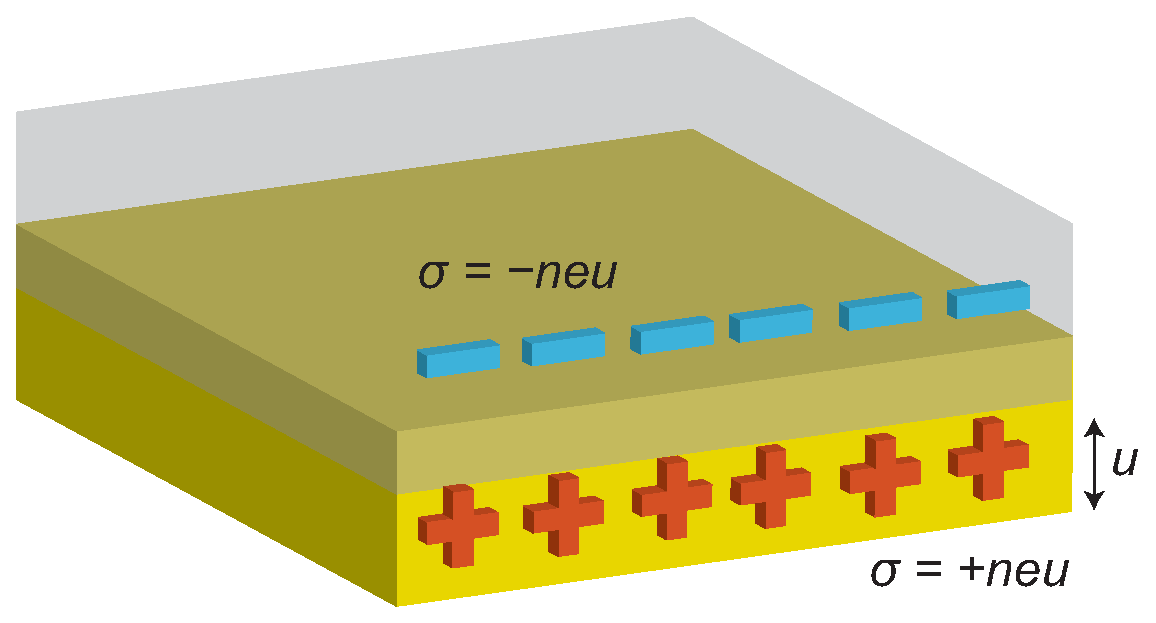
\includegraphics[scale=0.5]{THM/bulk.eps}
\caption{\label{fig:bulk}Longitudinal collective oscillations of the conduction electrons of a metal (Volume plasmons)}
\end{figure}

\begin{table}[!]\begin{center}
\caption{Table Example 1}
\begin{tabularx}{8cm}{llX}
\hline
Start & End  & Character Block Name \\
\hline
3400  & 4DB5 & CJK Unified Ideographs Extension A \\
4E00  & 9FFF & CJK Unified Ideographs \\
\hline
\end{tabularx}
 \end{center}\end{table}
 
\begin{figure}[!]
\centering
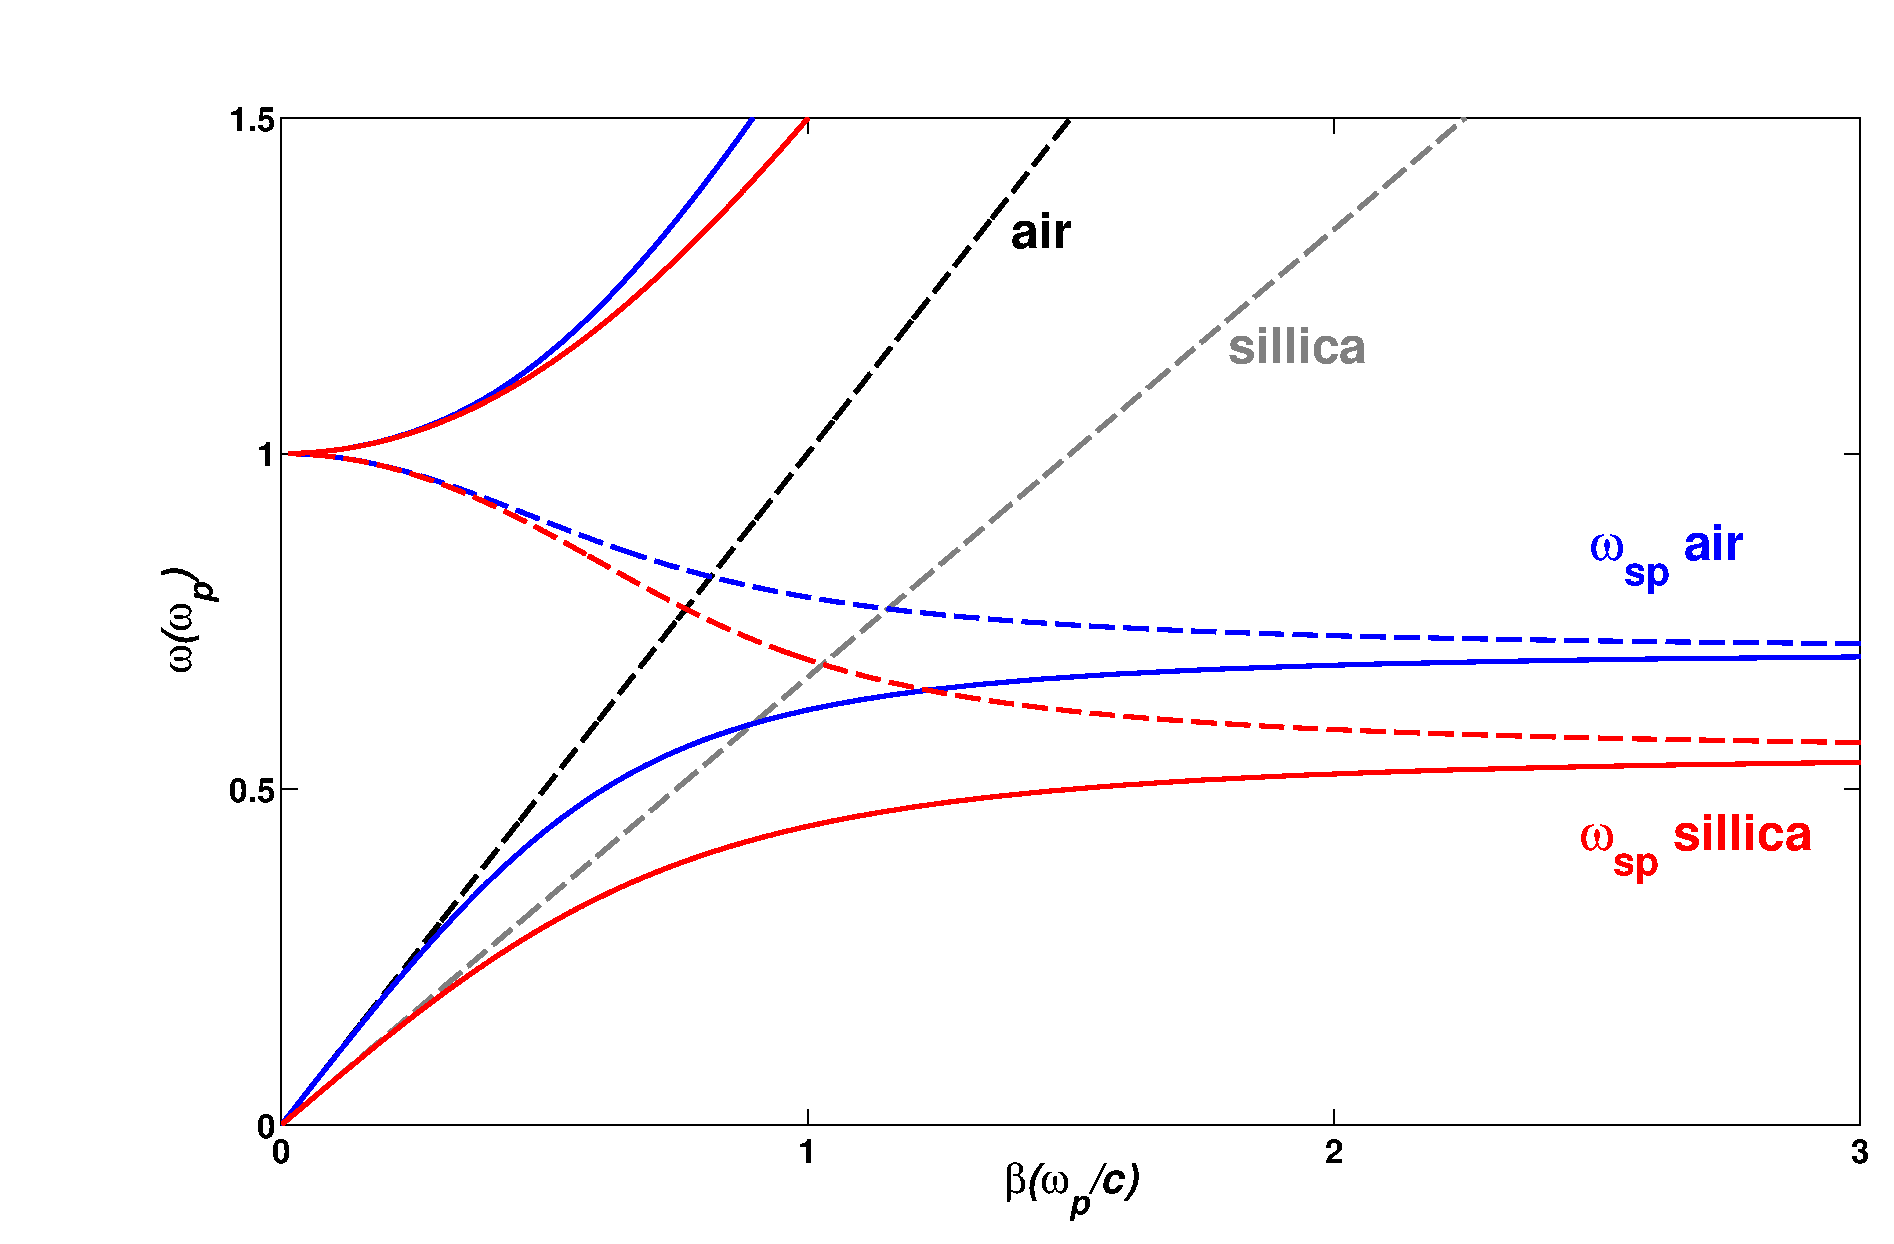
\includegraphics[scale=0.4]{THM/SPPdisp.eps}
\caption{\label{fig:SPPdisp}Dispersion relation of SPPs at the interface between a Drude metal with negligible collision frequency and air (blue curves) and silica (red curves).}
\end{figure}

\setcounter{chapter}{4}  %使章節couter切回4,第4章圖放在此行之後
\setcounter{figure}{1}  %使圖檔couter切回1

\begin{figure}[!]
\centering
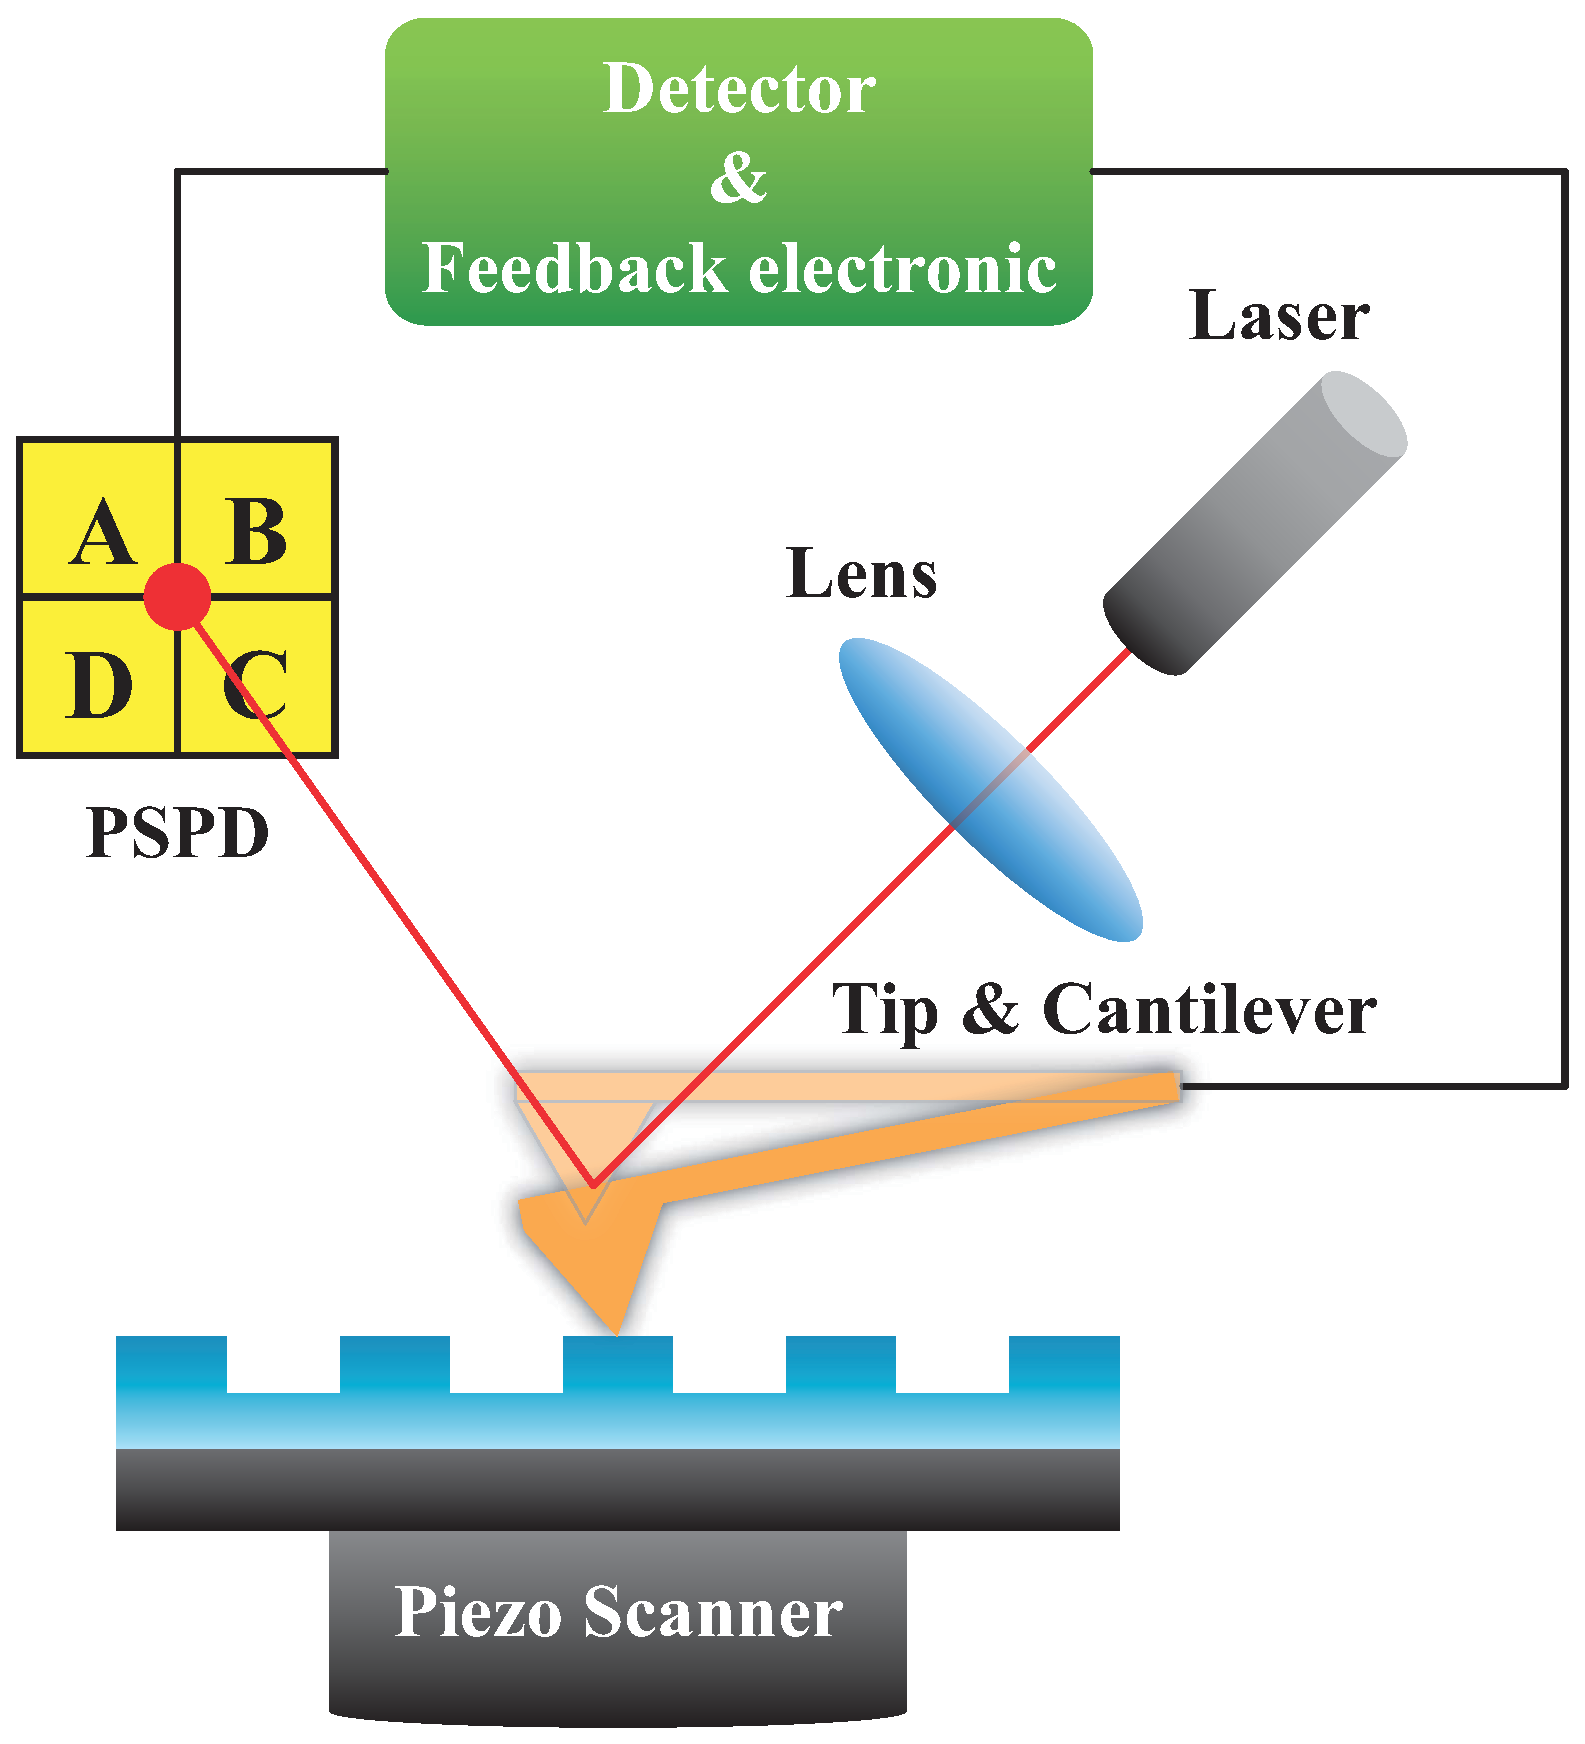
\includegraphics[scale=0.35]{EXP/afm1.eps}
\caption{\label{fig:afm1}Schematic of atomic force microscopy.}
\end{figure}

\begin{figure}[!]
\centering
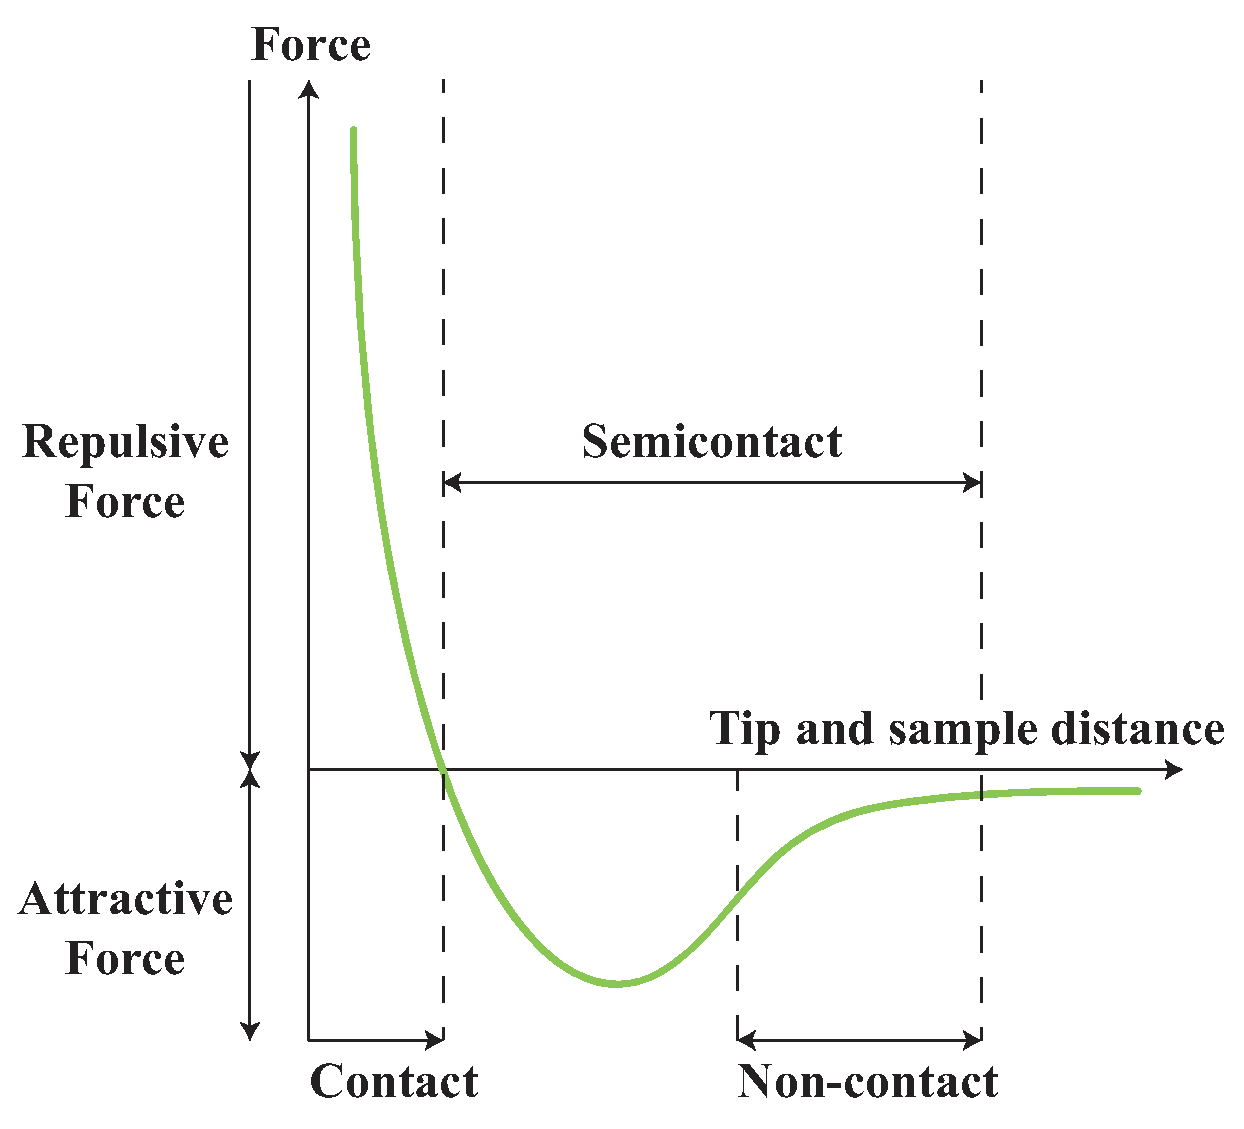
\includegraphics[scale=0.6]{EXP/afm3.eps}
\caption{\label{fig:afm3}Sketch of tip-sample forces.}
\end{figure}

%----------- 重新設定counter格式,章節的計數器格式為A…Z,圖檔和表格的格式皆為1…9 -----------
\renewcommand{\thefigure}{\Alph{chapter}.\arabic{figure}} 
\renewcommand{\thetable}{\Alph{chapter}.\arabic{table}}
%--------- Input your appendix figures and tables here  ---------
\setcounter{chapter}{3}%使章節couter切回3,附錄3圖放在此行之後
\setcounter{figure}{1}  %使圖檔couter切回1
\setcounter{table}{1}  %使表格couter切回1

\begin{figure}[!]
\centering
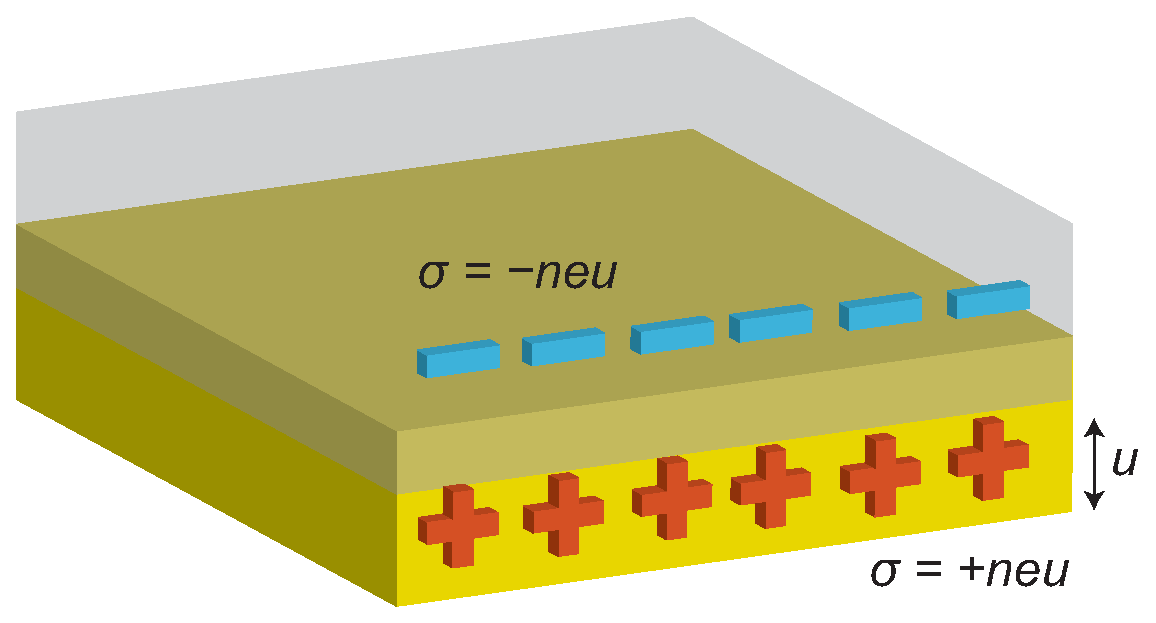
\includegraphics[scale=0.5]{THM/bulk.eps}
\caption{\label{fig:bulk}Longitudinal collective oscillations of the conduction electrons of a metal (Volume plasmons)}
\end{figure}

\begin{table}[!]\begin{center}
\caption{Table Example 1}
\begin{tabularx}{8cm}{llX}
\hline
Start & End  & Character Block Name \\
\hline
3400  & 4DB5 & CJK Unified Ideographs Extension A \\
4E00  & 9FFF & CJK Unified Ideographs \\
\hline
\end{tabularx}
\end{center}\end{table}

\begin{figure}[!]
\centering
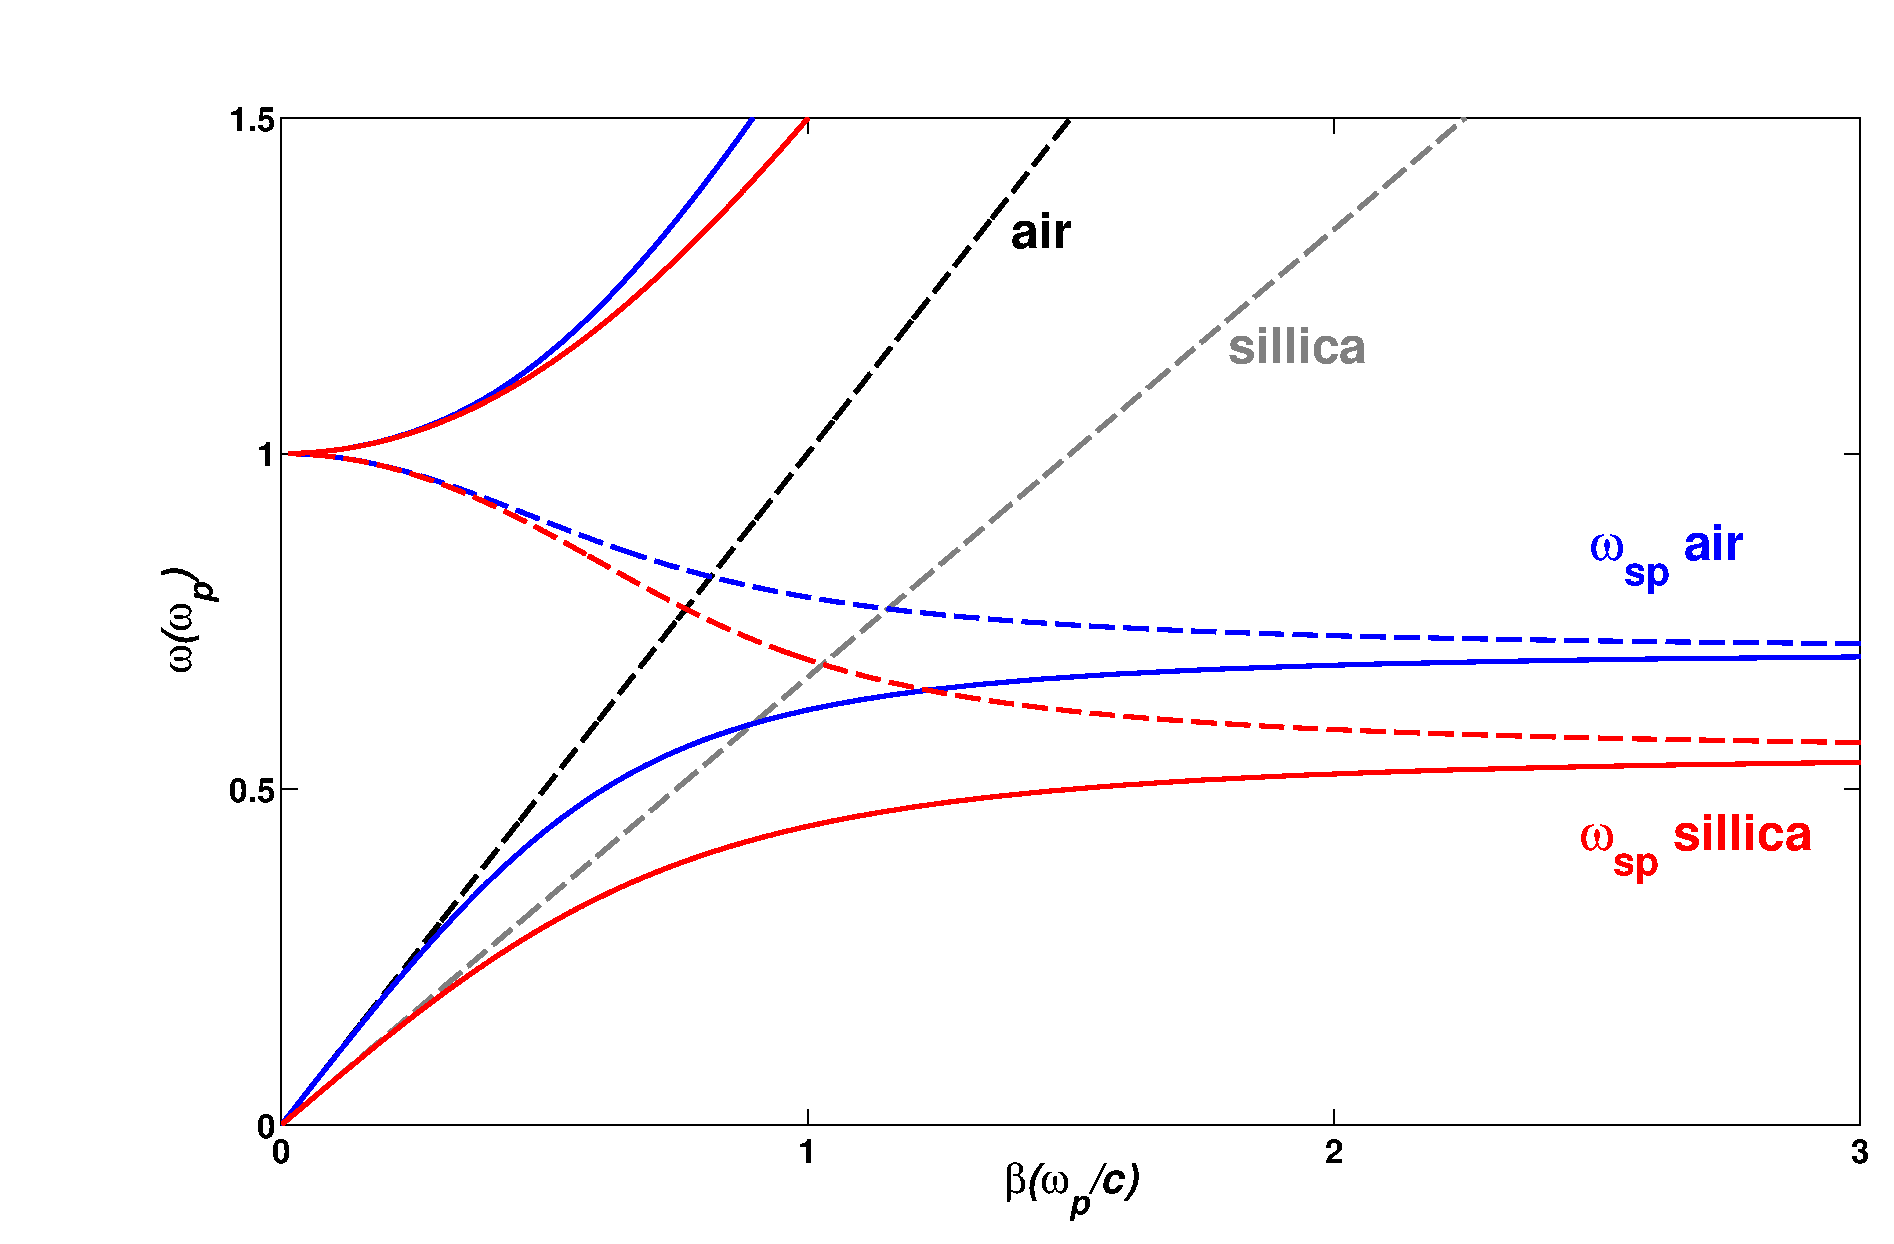
\includegraphics[scale=0.4]{THM/SPPdisp.eps}
\caption{\label{fig:SPPdisp}Dispersion relation of SPPs at the interface between a Drude metal with negligible collision frequency and air (blue curves) and silica (red curves).}
\end{figure}

\setcounter{chapter}{4}  %使章節couter切回4,附錄4章圖放在此行之後
\setcounter{figure}{1}  %使圖檔couter切回1

\begin{figure}[!]
\centering
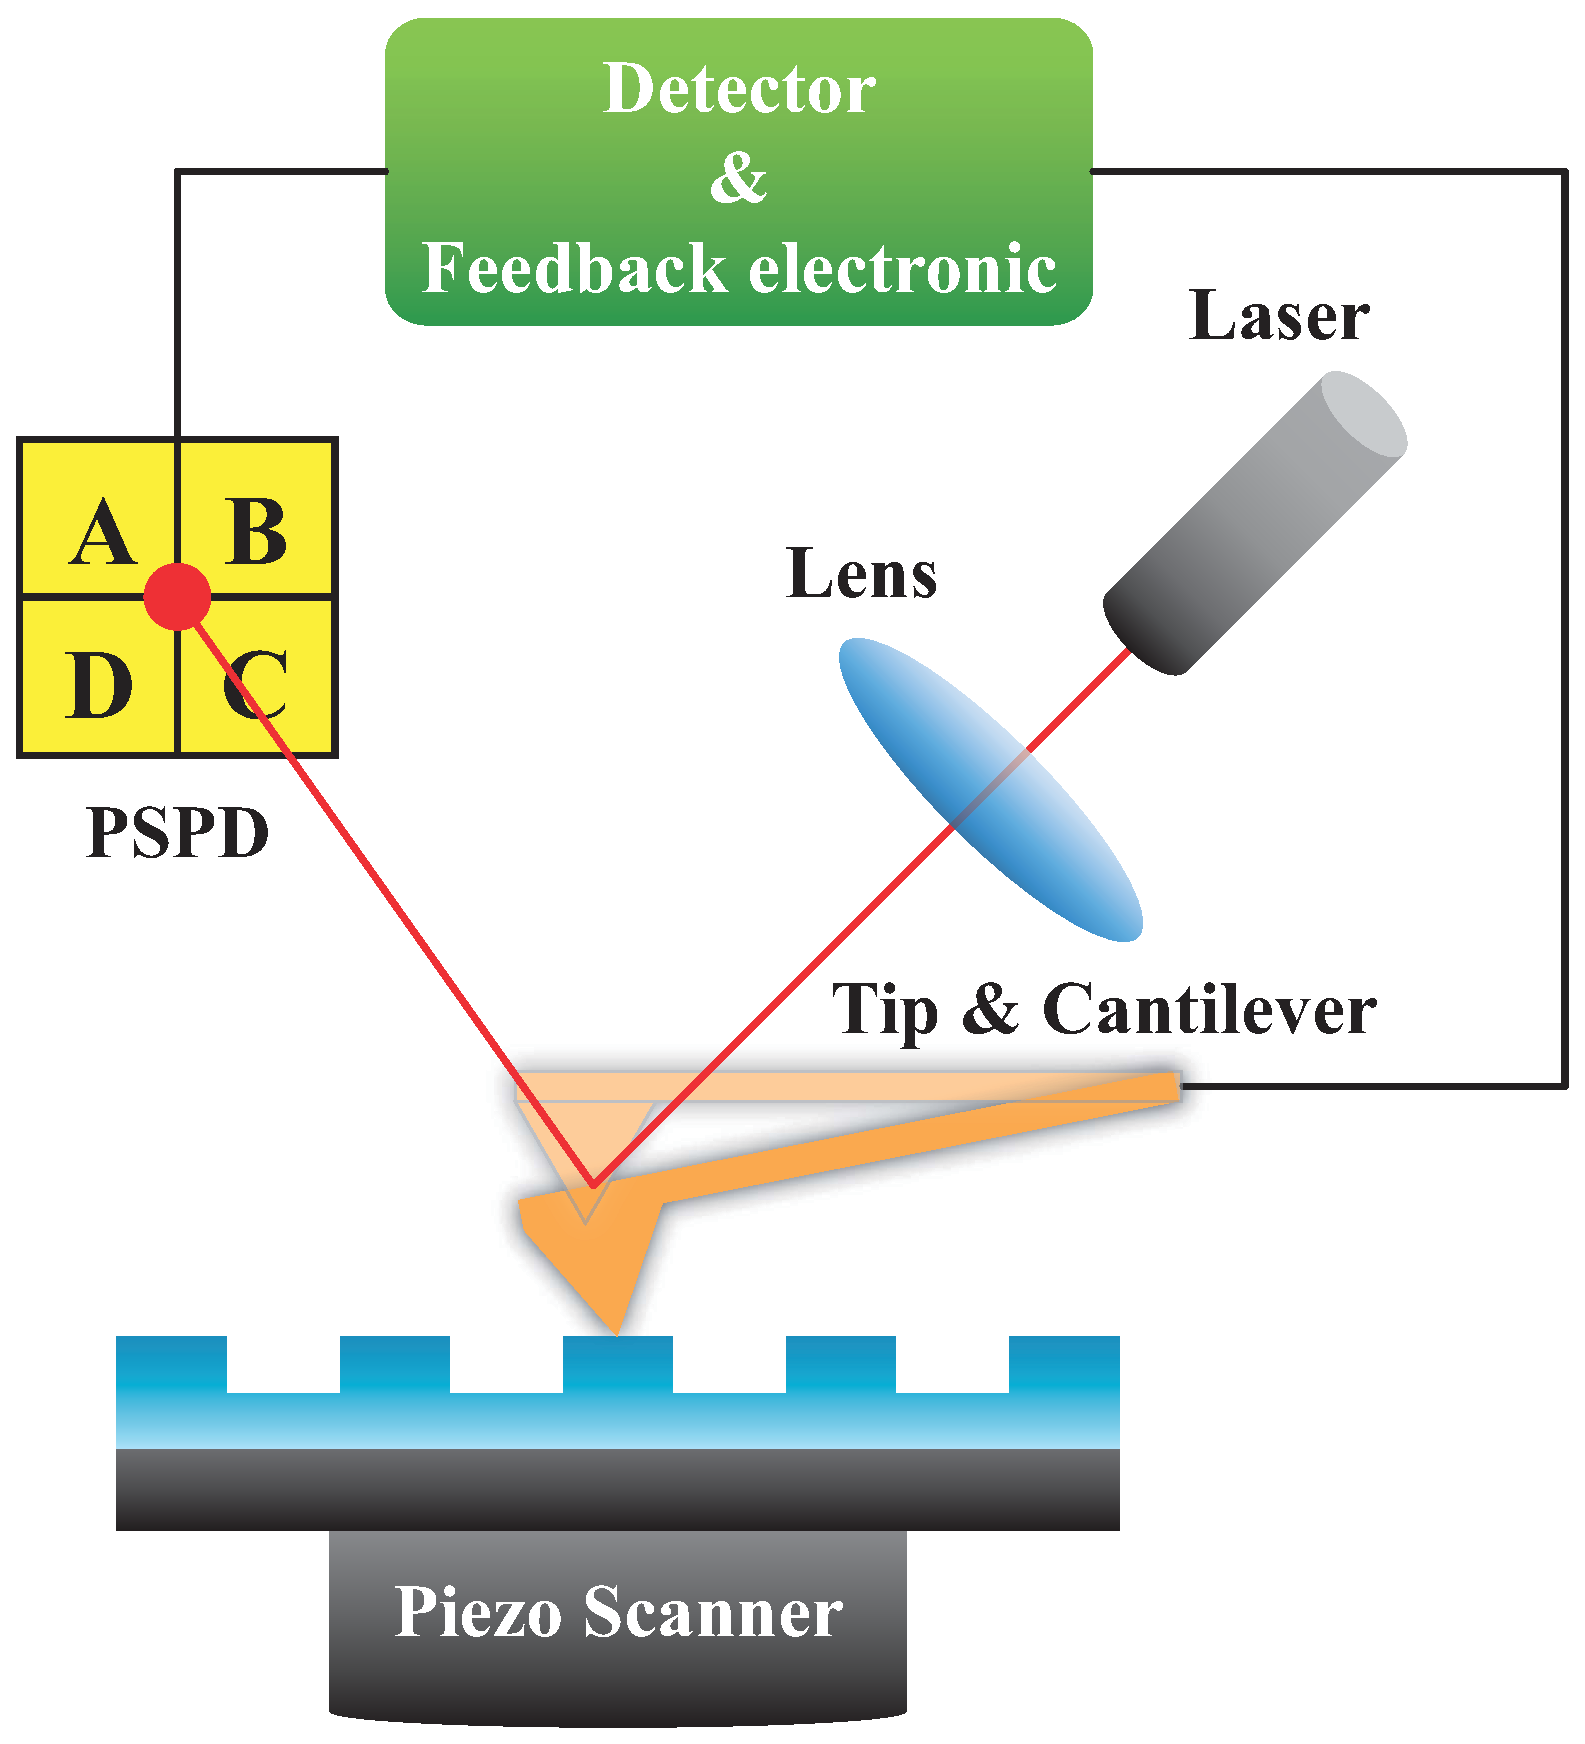
\includegraphics[scale=0.35]{EXP/afm1.eps}
\caption{\label{fig:afm1}Schematic of atomic force microscopy.}
\end{figure}

\begin{figure}[!]
\centering
\includegraphics[scale=0.6]{EXP/afm3.eps}
\caption{\label{fig:afm3}Sketch of tip-sample forces.}
\end{figure} 
%chapter cite  == \include
%\chapter*{}  %加星號隱藏標題

%----------- 重新設定counter格式,章節圖檔和表格的計數器格式皆為1…9 -----------
\renewcommand{\thefigure}{\arabic{chapter}.\arabic{figure}} 
\renewcommand{\thetable}{\arabic{chapter}.\arabic{table}} 
%--------- Input your main figures and tables here  ---------
\setcounter{chapter}{3}%使章節couter切回3,第三章圖放在此行之後
\setcounter{figure}{1}  %使圖檔couter切回1
\setcounter{table}{1}  %使表格couter切回1

\begin{figure}[!]
\centering
\includegraphics[scale=0.5]{THM/bulk.eps}
\caption{\label{fig:bulk}Longitudinal collective oscillations of the conduction electrons of a metal (Volume plasmons)}
\end{figure}

\begin{table}[!]\begin{center}
\caption{Table Example 1}
\begin{tabularx}{8cm}{llX}
\hline
Start & End  & Character Block Name \\
\hline
3400  & 4DB5 & CJK Unified Ideographs Extension A \\
4E00  & 9FFF & CJK Unified Ideographs \\
\hline
\end{tabularx}
 \end{center}\end{table}
 
\begin{figure}[!]
\centering
\includegraphics[scale=0.4]{THM/SPPdisp.eps}
\caption{\label{fig:SPPdisp}Dispersion relation of SPPs at the interface between a Drude metal with negligible collision frequency and air (blue curves) and silica (red curves).}
\end{figure}

\setcounter{chapter}{4}  %使章節couter切回4,第4章圖放在此行之後
\setcounter{figure}{1}  %使圖檔couter切回1

\begin{figure}[!]
\centering
\includegraphics[scale=0.35]{EXP/afm1.eps}
\caption{\label{fig:afm1}Schematic of atomic force microscopy.}
\end{figure}

\begin{figure}[!]
\centering
\includegraphics[scale=0.6]{EXP/afm3.eps}
\caption{\label{fig:afm3}Sketch of tip-sample forces.}
\end{figure}

%----------- 重新設定counter格式,章節的計數器格式為A…Z,圖檔和表格的格式皆為1…9 -----------
\renewcommand{\thefigure}{\Alph{chapter}.\arabic{figure}} 
\renewcommand{\thetable}{\Alph{chapter}.\arabic{table}}
%--------- Input your appendix figures and tables here  ---------
\setcounter{chapter}{3}%使章節couter切回3,附錄3圖放在此行之後
\setcounter{figure}{1}  %使圖檔couter切回1
\setcounter{table}{1}  %使表格couter切回1

\begin{figure}[!]
\centering
\includegraphics[scale=0.5]{THM/bulk.eps}
\caption{\label{fig:bulk}Longitudinal collective oscillations of the conduction electrons of a metal (Volume plasmons)}
\end{figure}

\begin{table}[!]\begin{center}
\caption{Table Example 1}
\begin{tabularx}{8cm}{llX}
\hline
Start & End  & Character Block Name \\
\hline
3400  & 4DB5 & CJK Unified Ideographs Extension A \\
4E00  & 9FFF & CJK Unified Ideographs \\
\hline
\end{tabularx}
\end{center}\end{table}

\begin{figure}[!]
\centering
\includegraphics[scale=0.4]{THM/SPPdisp.eps}
\caption{\label{fig:SPPdisp}Dispersion relation of SPPs at the interface between a Drude metal with negligible collision frequency and air (blue curves) and silica (red curves).}
\end{figure}

\setcounter{chapter}{4}  %使章節couter切回4,附錄4章圖放在此行之後
\setcounter{figure}{1}  %使圖檔couter切回1

\begin{figure}[!]
\centering
\includegraphics[scale=0.35]{EXP/afm1.eps}
\caption{\label{fig:afm1}Schematic of atomic force microscopy.}
\end{figure}

\begin{figure}[!]
\centering
\includegraphics[scale=0.6]{EXP/afm3.eps}
\caption{\label{fig:afm3}Sketch of tip-sample forces.}
\end{figure}
    \end{verbatim}
    在章節檔\href{run:./EndFigTab.tex}{EndFigTab.tex}裡有範例和說明可供參考,要注意正文的圖表和附錄的圖表要分清楚,即在\href{run:./EndFigTab.tex}{EndFigTab.tex}內
    \begin{verbatim}    
\renewcommand{\thefigure}{\arabic{chapter}.\arabic{figure}} 
\renewcommand{\thetable}{\arabic{chapter}.\arabic{table}} 
%--- Input your main figures and tables here  ---
    \end{verbatim}
    這幾行之後章節計數器格式已切換為1\dots 9,放正文的圖表 ,
     \begin{verbatim}    
\renewcommand{\thefigure}{\Alph{chapter}.\arabic{figure}} 
\renewcommand{\thetable}{\Alph{chapter}.\arabic{table}}
%--- Input your appendix figures and tables here  ---
    \end{verbatim}
    這幾行之後章節計數器格式已切換為A\dots Z,放附錄的圖表。另外要取消圖表的浮動功能,才能讓圖表按照指令出現順序排好,即把平常使用的圖表指令
    \begin{verbatim}    
\begin{figure}[htb]
...
\begin{table}[htb]
    \end{verbatim}
    改成
     \begin{verbatim}    
\begin{figure}[!]
...
\begin{table}[!]
    \end{verbatim}
    剩下的只要注意章節圖表的計數器設定即可。\texttt{\textbackslash ref}和\texttt{\textbackslash label}指令可以在此圖表章節與正文章節使用。
     \item 如果我想要修改margin(文字邊界)的話,可以從哪裡下手呢?\\
     請打開\href{run:./ntu.sty}{ntu.sty}修改下面這行的上下左右參數即可:
    \begin{verbatim}
\RequirePackage[top=3cm,left=3cm,bottom=2cm,right=3cm]{geometry}
    \end{verbatim}
    \item 我想引用Twomey (1974): Pollution and planetary albedo這篇論文,如何用\texttt{\textbackslash cite}引用它的時候在內文顯示Twomey (1974) [編號] ?\\
    建議使用natbib套件,參考資料如下:\\
    \href{http://en.wikibooks.org/wiki/LaTeX/Bibliography_Management}{LaTeX/Bibliography Management}\\
    \href{http://nodonn.tipido.net/bibstyle.php}{Overview of Bibtex-Styles}\\
    \href{http://merkel.zoneo.net/Latex/natbib.php}{Reference sheet for natbib usage }\
 \item \XeTeX\ :\\
    此範本中文字體使用\XeTeX\ 轉換,細節請參考\href{http://www.hitripod.com/blog/}{Hitripod}寫的\href{http://www.hitripod.com/blog/2011/04/xetex-chinese-font-cjk-latex/}{ 
XeTeX:解決 LaTeX 惱人的中文字型問題}。
 \item 如何輸入英文`單引號'和``雙引號''以及不同長度的破折號?\\
        可以參考\href{run:./latex123.pdf}{李果正-大家來學\LaTeX}第17頁針對標點符號的遊戲規則,範例如下,輸入以下指令:\\
        \begin{verbatim}
`單引號'\\
``雙引號''\\
-hyphen\\
--en-dash\\
---em-dash\\
        \end{verbatim} 
        則顯示:\\
       `單引號'\\
        ``雙引號''\\
        -hyphen\\
        --en-dash\\
        ---em-dash\\
    \end{enumerate} 
    \end{enumerate} 
               

%----------- Have a fractal fern? -----------
%\begin{pspicture}
%\psFern[scale=30,maxIter=100000,linecolor=Green]
%\end{pspicture}

 \end{acknowledgementsCH}